% =====================================================================
% Experimental Astronomy (Springer) journal layout -- EMULATED.
% Compile with XeLaTeX (e.g. latexmk -pdfxe).
% Auto-generated from the NIM-A elsarticle source by build_ea_format.py;
% only the journal FORMAT changed -- text, figures, tables, and references
% are carried over verbatim from balloon511_nima_draft_zh.tex.
% For submission, replace this emulated preamble with the official Springer
% Nature class (sn-jnl.cls); the structure is already aligned to it.
% =====================================================================
\documentclass[11pt]{article}
\usepackage[a4paper,top=2.4cm,bottom=2.5cm,left=2.0cm,right=2.0cm]{geometry}
\usepackage{amsmath,amssymb}
\usepackage[UTF8]{ctex}
\usepackage{fontspec}
\setmainfont{TeX Gyre Termes}
\usepackage{booktabs}
\usepackage{graphicx}
\usepackage{pdflscape}
\usepackage[section]{placeins}
\graphicspath{{./}}
\renewcommand{\topfraction}{0.92}
\renewcommand{\bottomfraction}{0.8}
\renewcommand{\textfraction}{0.07}
\renewcommand{\floatpagefraction}{0.75}
\usepackage{xcolor}
\usepackage{tikz}
\usetikzlibrary{arrows.meta,positioning}
\usepackage{caption}
\captionsetup{font=small,labelfont=bf}
\usepackage{titlesec}
\titleformat{\section}{\normalfont\large\bfseries}{\thesection}{0.6em}{}
\titleformat{\subsection}{\normalfont\normalsize\bfseries}{\thesubsection}{0.5em}{}
\titleformat{\subsubsection}{\normalfont\normalsize\bfseries}{\thesubsubsection}{0.5em}{}
\titlespacing*{\section}{0pt}{1.3ex plus .2ex minus .2ex}{0.6ex}
\titlespacing*{\subsection}{0pt}{1.0ex plus .2ex minus .2ex}{0.5ex}
\usepackage{fancyhdr}
\pagestyle{fancy}
\fancyhf{}
\fancyhead[L]{\small\itshape Experimental Astronomy}
\fancyhead[R]{\small\thepage}
\renewcommand{\headrulewidth}{0.4pt}
\usepackage{cite}
\usepackage{hyperref}
\hypersetup{hidelinks}
\setlength{\emergencystretch}{3em}
\newcommand{\keV}{\,\mathrm{keV}}
\newcommand{\MeV}{\,\mathrm{MeV}}
\newcommand{\cms}{\,\mathrm{cm^{-2}\,s^{-1}}}
\newcommand{\phcms}{\,\mathrm{ph\,cm^{-2}\,s^{-1}}}
\newcommand{\cps}{\,\mathrm{s^{-1}}}
\newcommand{\wii}{W_{511}}
\newcommand{\aeff}{A_{\mathrm{eff}}}
\newcommand{\fzero}{F_{0}}
\newcommand{\fthree}{F_{3\sigma}}

\begin{document}
\thispagestyle{fancy}
\begin{flushleft}
{\LARGE\bfseries 气球载 511 keV Laue 透镜 TES 望远镜本底和未分辨线灵敏度的探测器耦合 Monte Carlo 估计 \par}
\vspace{1.1em}
{\large 作者信息暂隐\par}
\vspace{0.3em}
{\normalsize\itshape 单位信息暂隐\par}
\end{flushleft}
\vspace{0.7em}
\noindent\rule{\textwidth}{0.4pt}
\vspace{0.5em}

\noindent\textbf{摘要}\hspace{0.7em}
本底决定气球载 511 keV Laue 透镜--过渡边缘传感器（TES）微量热计望远镜的灵敏度。本文采用端到端 Geant4/MEGAlib 链，分别处理聚焦天体信号、具有正确总动能轴的八族大气粒子场，以及按实际产生位置抽样的活化衰变。宽带大气光子场本身已包含湮没特征，因而只计数一次，不再叠加独立大气单能分量。全部计算流统一施加 $510.58$--$511.42\keV$ 科学窗、主动反符合以及拓扑/视场选择。SG3 参考几何第 15 天成熟本底为 $5.1280\times10^{-2}\cps$，其选后延迟率中有 $32.18\%$ 来自稀释制冷机混合室及各级冷盘。由该产生位置分布出发，SH3 将六层 TES 焦面横向移入主动 BGO 包围的铝烟囱，使冷端区域占比降至 $3.92\%$。选后有效面积仅由 $15.12324\pm0.04492$ 变为 $15.08544\pm0.04503\,\mathrm{cm^2}$，而第 15 天成熟本底由 $5.1280\times10^{-2}$ 降至 $9.280\times10^{-3}\cps$。在大气层顶 $10^{-4}\phcms$ 线流量下，SH3 第 15 天信号率为 $9.7904\times10^{-4}\cps$。固定 $45^\circ$ 仰角的 20 d 轨迹折叠得到 1678.14 个信号和 15551.68 个本底计数，高斯与 Asimov 显著度分别为 13.46 和 13.22，高斯 $3\sigma$ 流量阈值为 $(2.229\pm0.209)\times10^{-5}\phcms$。相对 SG3，SH3 保留 $99.75\%$ 的有效面积，将本底降至 $18.10\%$，最小可分辨流量改善约 2.43 倍。

\vspace{0.7em}
\noindent\textbf{关键词}\hspace{0.7em}伽马射线仪器 $\cdot$ 511 keV 湮灭线 $\cdot$ 过渡边缘传感器微量热计 $\cdot$ Laue 透镜 $\cdot$ 气球载望远镜 $\cdot$ Monte Carlo 本底模拟

\vspace{0.3em}
\noindent\rule{\textwidth}{0.4pt}
\vspace{1.0em}

\section{引言}
\label{sec:intro}

银河系 511 keV 湮灭辐射是研究银河系正电子产生、传播和湮灭环境的重要观测探针。其谱学特征包括接近 511 keV 的双光子谱线和位于较低能量处的正电子素连续谱。正电子可与电子直接湮灭，或先形成对位正电子素并产生两个约 511 keV 光子；正交正电子素则通过三光子衰变形成连续谱。因此，谱线强度、轮廓和正电子素连续谱可以约束正电子减速和湮灭所在介质的性质 \cite{Prantzos2011,Jean2006}。在近似稳态假设下，INTEGRAL/SPI 测得的银河系 511 keV 总通量对应约几 $\times10^{43}\,\mathrm{e^+\,s^{-1}}$ 的正电子湮灭率 \cite{Prantzos2011,Kierans2020}。候选正电子来源包括恒星爆发中合成的 $\beta^+$ 不稳定核素、能够产生正负电子对的致密天体，以及更具推测性的粒子物理情景，例如由轻质量暗物质湮灭或衰变注入低能正电子。现有观测尚不能唯一确定其中的主导贡献 \cite{Prantzos2011,Siegert2016AA,Siegert2016V404}。

过去的宽视场观测已经建立了 511 keV 辐射的弥散形态。INTEGRAL/SPI 显示出明亮的中心核球成分和较弱的银盘成分，20 年数据分析进一步重建出中心、宽核球与银盘结构，但额外关联结构的证据仍较边际 \cite{Knodlseder2005AllSky,Siegert2016AA,Yoneda2025}。COSI 2016 年气球飞行独立探测到核球信号，并给出辐射比单一点源更延展的迹象 \cite{Kierans2020,Siegert2020COSI}。谱学测量还约束了湮灭介质的物理状态和运动学：SPI 谱线可分解为约 $1.3\keV$ FWHM 的窄成分和约 $5.4\keV$ 的宽成分，并已在银河系内区搜寻其中心能量与线宽的变化 \cite{Jean2006,Siegert2019Kinematics}。然而，511 keV 天图记录的是正电子减速并湮灭后的位置，不一定是正电子最初产生的位置；正电子在热化之前可在磁化的多相星际介质中传播。因此，现有弥散形态和谱学约束仍不能单独判定主导来源，或还原湮灭前的输运历史 \cite{Prantzos2011}。

宽视场康普顿和编码孔径仪器非常适合测量核球和银盘的总体发射。为了检验中心区域是否还包含未分辨中心增强、紧致源或可测量的谱线运动学结构，需要一种互补的定点仪器。探测到点状或窄集中分布的特征，将表明部分湮灭在空间上是局域的；未探测到信号则会限制紧致成分，但不能排除正电子逃逸后以弥散形式湮灭的源族。INTEGRAL/IBIS 紧致源搜索未发现银河系 511 keV 点源，并针对银河系中心方向约 10 Ms 的曝光给出约 $1.6\times10^{-4}\phcms$ 的 $2\sigma$ 上限 \cite{DeCesare2011}。该上限既给出了以往紧致源搜索的比较尺度，也构成新型窄视场定点仪器的灵敏度目标。

Laue 光学利用透射式 Bragg 衍射，将来自已知方向的光子聚焦到小型焦面上，为这种定点观测提供了一种途径 \cite{Barriere2009Laue,Barriere2011LauePrototype}。当探测器相关本底占主导时，把大口径收集的通量汇聚到较小的灵敏探测器面积上，可以提高点源灵敏度 \cite{Weidenspointner2006MAX}。相应的焦面必须兼具窄能量响应和足够的 511 keV 阻止效率。过渡边缘传感器（transition-edge sensor, TES）微量热计利用超导体陡峭的电阻转变测量沉积能量引起的微小温度变化，可在 511 keV 处提供亚 keV 能量分辨率 \cite{Shirazi2023,Zhang2022TESGamma}。阵列用于覆盖焦斑，厚吸收体与多层布局则提高全能量效率。Laue 聚焦压缩接收相空间，而 TES 响应允许使用窄线窗并进行精细谱线轮廓测量。所得仪器以视场换取集中束流和高分辨率谱学能力，是对核球和银盘宽视场测量的补充，而不是替代。

不过，TES 探测器本征的高能量分辨率和聚焦光学的聚焦性能并不足以单独论证整套探测系统针对点源的高分辨率 \cite{Shirazi2023,Hu2026}。大气环境中的宇宙线本底在探测器灵敏区沉积的瞬发本底谱，以及宇宙线在探测器及探测器周围物质活化引起的次级延时本底谱，也会影响探测系统对于科学源探测的分辨能力 \cite{Gallego2025Balloon,Tian2026DIXE}。

本工作旨在量化球载 Laue 透镜--TES 阵列望远镜系统在高空环境下对于银河系中心 511 keV 点源的探测性能，同时研判本底的来源与分布，给出进一步设计优化的指导意见。

\subsection{科学目标与仪器要求}
\label{sec:requirements}

\begingroup
\clubpenalty=10000
\widowpenalty=10000

本文模拟的仪器旨在探测此前仪器尚未发现的银河系中心区域 511 keV 点源或未分辨中心超额成分。INTEGRAL/SPI 测量表明，511 keV 天空辐射以弥散的核球和银盘发射为主 \cite{Siegert2016AA,Yoneda2025}。De Cesare 针对 INTEGRAL/IBIS 开展的紧致源专项搜索未发现银河系 511 keV 点源，并给出了银河系中心方向 10 Ms 曝光下的 $2\sigma$ 上限 \cite{DeCesare2011}。为与本文报告的 $3\sigma$ 灵敏度进行比较，我们在高斯近似下对该已发表上限作线性换算，得到基于 IBIS 结果的 $3\sigma$ 等效大气层顶上限 $2.4\times10^{-4}\phcms$。在飞行第 15 天的高度，保留的垂直剩余大气柱深为 $3.461\,\mathrm{g\,cm^{-2}}$。对于本文设计的固定 $45^\circ$ 仰角仪器轴，平面平行近似下的斜程柱深为 $4.895\,\mathrm{g\,cm^{-2}}$；采用与 NIST XCOM 在 511 keV 附近数据一致的有效干空气衰减系数 $0.08736\,\mathrm{cm^2\,g^{-1}}$，得到透过率 $T_{15,45}=0.6520$。施加该透过率后，定义唯一的载荷平面观测参考通量 $F_{0,\mathrm{ref}}=(2.4\times10^{-4})\times0.6520=1.565\times10^{-4}\phcms$。该参考通量将作为后文评估所模拟望远镜系统在可接受飞行时间内最小可分辨通量性能的参照。与 INTEGRAL 已开展的宽视场光谱和编码孔径搜索相比，本文模拟的载荷引入 Laue 聚焦以改善点源响应，并采用高能量分辨率、多层厚吸收体 TES 微量热计阵列作为焦面探测器，以提高 511 keV 谱线测量能力 \cite{Shirazi2023,Caputo2017}。

本工作首先考虑早期测试用的气球载荷平台，并期望后续拓展到卫星观测平台。

\begingroup
\interlinepenalty=10000
这一目标对仪器和模拟提出四项要求。第一，望远镜必须将大口径透镜收集的 511 keV 光子汇聚到小型焦面上，从而提高聚焦光学的集光面积与探测器灵敏面积之比；这是一种窄视场定点构型，而不是扩大天空覆盖范围的手段。第二，焦面探测器必须具备足以分辨精细谱线结构的亚 keV 能量响应。第三，探测器和屏蔽模型必须抑制大气本底、活化本底及侧向入射本底。第四，模拟链必须一致处理瞬发本底、延迟活化、聚焦信号、veto、事例拓扑及任务时间变化，使信号和本底在相同的探测器选择条件下进行评估。
\par
\endgroup

本文余下结构如下：第 2 节给出探测器与低温系统质量模型；第 3 节描述模拟框架——模拟流程、光学耦合、本底来源、事例选择，以及任务时间轨迹折叠（第~\ref{sec:mission_time_fold}~小节）；第 4 节给出选后率和灵敏度结果以及归一化、收敛与边界检查；第 5 节为讨论与结论。

\endgroup

\section{探测器与低温系统质量模型}
\label{sec:geometry}

本文采用现行 SG3 探测器--低温系统几何作为可审计参考。该几何包含安装在小型稀释制冷机混合室和多级冷盘下方的六层 TES 阵列，以及热屏蔽、磁屏蔽、铜支撑、侧入射窗口、钨准直器、主动闪烁体和低温服务结构 \cite{Shirazi2023,Gottardi2021TESReview}。图~\ref{fig:mass_model} 以精确截面连接参考焦面布置与选后本底分析。第~\ref{subsec:optimized_shield_results_zh}~小节引入的 SH3 侧烟囱几何保留相同探测器、光学、响应和源约定，使几何比较严格同口径。

TES 探测器概念采用本实验室研发的 AlMn 薄膜与吸收体耦合结构。AlMn 合金的相变温度可通过成分和退火工艺调节，适于阵列制备，并且对磁场相对不敏感 \cite{Xie2026AlMn,Vavagiakis2017AlMnMagnetic}。在本文概念设计中，TES 温度计为厚约 $200\,\mathrm{nm}$、名义 Mn 原子浓度为 $2000\,\mathrm{ppm}$ 的 AlMn 薄膜，而 $\gamma$ 射线吸收体为毫米量级金属体。吸收体采用 $1.5\times1.5\times3.0\,\mathrm{mm^3}$ Ta 像素；Ta 的高原子序数提高了 511 keV 光子的相互作用效率。在 511 keV 处，单层 $3.0\,\mathrm{mm}$ Ta 的预估相互作用效率约为 $49\%$，相应的六层效率接近 1。当前几何中，相邻 Ta 阵列层的中心间距为 $12\,\mathrm{mm}$；该间距的设计兼顾后续基于康普顿运动学轨迹重建的 veto 机制。选择 Ta 还考虑了其作为超导体在低温下较低的体积热容（本文采用 $10^{-2}\,\mathrm{J\,K^{-1}\,m^{-3}}$ 的量级估计）及其较高的光电--康普顿相互作用比。根据 NIST XCOM 在 511 keV 附近的截面，该比值约为 0.731 \cite{NISTXCOM}。在探测器响应模型中，我们根据本实验室已开发的 X 射线 TES 的实验经验 \cite{Xie2026AlMn}，采用 $\Delta E_{\mathrm{FWHM}}\simeq420\,\mathrm{eV}$ 作为 511 keV 处的预估能量分辨率和探测器响应后处理输入。

由于 TES 薄膜与 Ta 吸收体在尺寸和质量上相差很大，且 TES 薄膜本身对 511 keV 光子的相互作用贡献可忽略，输运几何使用 Ta 吸收体代表 TES 像素的主要敏感体积。显式建模的敏感体积共 6 层，每层包含 376 个 Ta 吸收体像素，总计 2256 个像素；每个像素长、宽均为 $1.5\,\mathrm{mm}$，厚度为 $3\,\mathrm{mm}$。每个 Ta 像素下方放置一个 Si 衬底代理；由于本模拟不处理详细热传导，使用 Si 代表 $\mathrm{SiO_2}$--$\mathrm{SiN_x}$--Si 衬底。TES 薄膜、布线和读出细节不作为显式相互作用体积逐层建立，而是通过假设的能量响应和服务质量代理进入模型。与响应 FWHM 独立定义，保留的科学窗选择采用 511 keV 线窗 $W_{511}=511\,\mathrm{keV}\pm420\,\mathrm{eV}$，即 $510.58$--$511.42\,\mathrm{keV}$。

SG3 的 TES 阵列安装在多级冷盘正下方的铜支架上。沿光路依次设置铝热屏蔽窗、Be 真空窗和与 TES 像素对准的 W 多孔准直器；周围壳层通过布尔开孔形成侧入射光路。完整仪器框架旋转 $45^\circ$，使局部孔径在地平坐标中指向 $45^\circ$ 仰角。

优化后的 SH3 保留六层 TES 和上游光学接受度，但把焦面横向平移到圆柱形铝烟囱中。烟囱内、外半径分别为 10.75 和 11.05 cm，壁厚 3 mm，共同局部轴为 $z'=-2.80$ cm。紧凑 W 框支撑焦面，主动 BGO 覆盖烟囱侧面、前端光学环和后端冷孔环。三个主动 BGO 体积的能量沉积按事例求和；原生触发参考为 $80\keV$，而下文共同离线反符合门要求 BGO 总沉积严格低于 $50\keV$。

\begin{figure}[t]
\centering
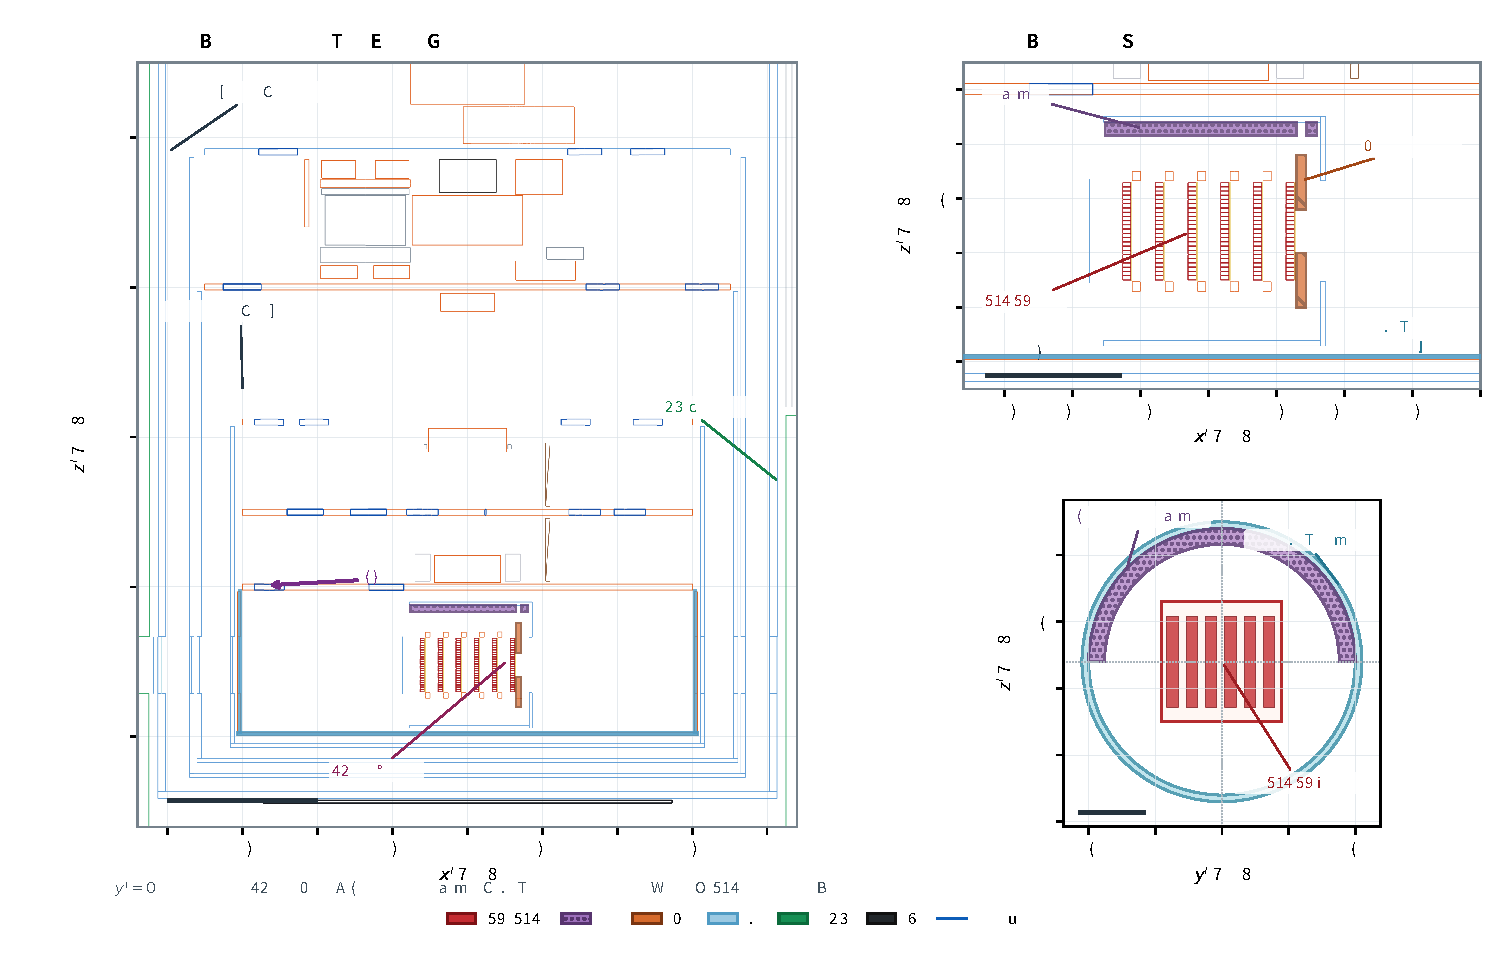
\includegraphics[width=0.98\linewidth]{figures/fig01_sg3_detailed_mass_model_zh.pdf}
\caption{现行 SG3 参考探测器--低温系统质量模型。（a）精确 $y'=0$ 全局网格截面，显示外部承力结构、真空包络、多级低温屏、主动 BGO 与探测器舱；箭头标出固定 $45^\circ$ 天空指向。（b）探测器舱放大截面，显示六层 TES、Cu 环形热连接、Bi 半圆筒和 Al 冷端包络。（c）垂直烟囱轴的横截面，给出 4.796 mm Bi 半圆筒、2 mm Al 圆筒与六个 TES Ta 吸收体的遮蔽关系。}
\label{fig:mass_model}
\end{figure}

图~\ref{fig:mass_model} 的质量模型截面来自保留的三角网格，而不是简化探测器卡通图。全局面板把真空包络、承力壳、多级热屏、服务贯穿件、主动 BGO、冷盘和探测器舱放在同一仪器坐标中；近场面板则解析直接影响 511 keV 本底的六个 Ta 吸收体平面、Cu 支撑与热沉连接、Al 冷端包络及焦面上方的 Bi 构件。SG3 的 Bi 构件是紧贴保留 2 mm Al 圆筒内侧的 4.796 mm 上半圆筒，既保留连续光学开口，也避免把吸收体误解为无限延伸的平板。

三个面板还分开了后文分析中的两个几何问题。全局截面确定哪些大质量载荷结构可以产生或散射进入低温系统的粒子；两个近场截面则确定活化结构在产生之后对 TES 张开的立体角。选后来源分析使用同一生成几何对应的体积名称和坐标，而不是人工划定的径向区域。因此，归因于混合室板、Cu 环或 TES 近场构件的延迟事例可以直接放回质量模型，且不需要变换坐标约定。这一“源--几何”对应关系使“载荷中存在的活度”与“能够耦合进科学窗的活度”得到区分。

SG3 和 SH3 保留相同的六个敏感平面、像素尺寸、响应模型、入射孔径和光轴约定；受控变化只是焦面与冷端结构的相对位置。SG3 中 TES 位于冷端投影下方，SH3 中则沿侧烟囱轴布置，背靠紧凑局部框并处于主动 BGO 包络内。固定探测器和光学定义至关重要，否则本底下降无法与聚焦接受度同时损失的情形分离。

\FloatBarrier

\section{模拟框架}
\label{sec:framework}

通过详细质量模型的探测器耦合 Monte Carlo 输运，是预测伽马射线谱仪响应和本底的成熟方法 \cite{Sturner2003}。光学分支在 Laue 透镜中输运轴上 511 keV 点源并记录焦面相空间；探测器分支则独立处理三条物理链：由该相空间得到的聚焦 EventList、经正确能量轴修复的宽带大气场，以及从记录产生位置发射的放射性衰变。活化产生只是延迟链的源构建阶段，不作为瞬发计数分量。三条链统一施加像素响应、科学窗、主动 BGO 反符合和拓扑/视场选择，选后率再进入公共时间轴与同一条 81 节点轨迹。

图~\ref{fig:workflow} 保留成熟的“源--输运--响应--选择--任务折叠”结构，并明确当前源约定：宽带大气光子表已经包含 511 keV 附近的湮没特征，不再加入独立大气单能线。随后以选后事例的粒子族、母核素、材料体积和产生位置分解 SG3 参考本底，并在相同约定下比较 SH3 侧烟囱。日尺度飞行连续采样大气与地磁状态，任务轨迹折叠及五个公共时间锚点见第~\ref{sec:mission_time_fold}~小节。

\begin{landscape}
\centering
\vspace*{\fill}
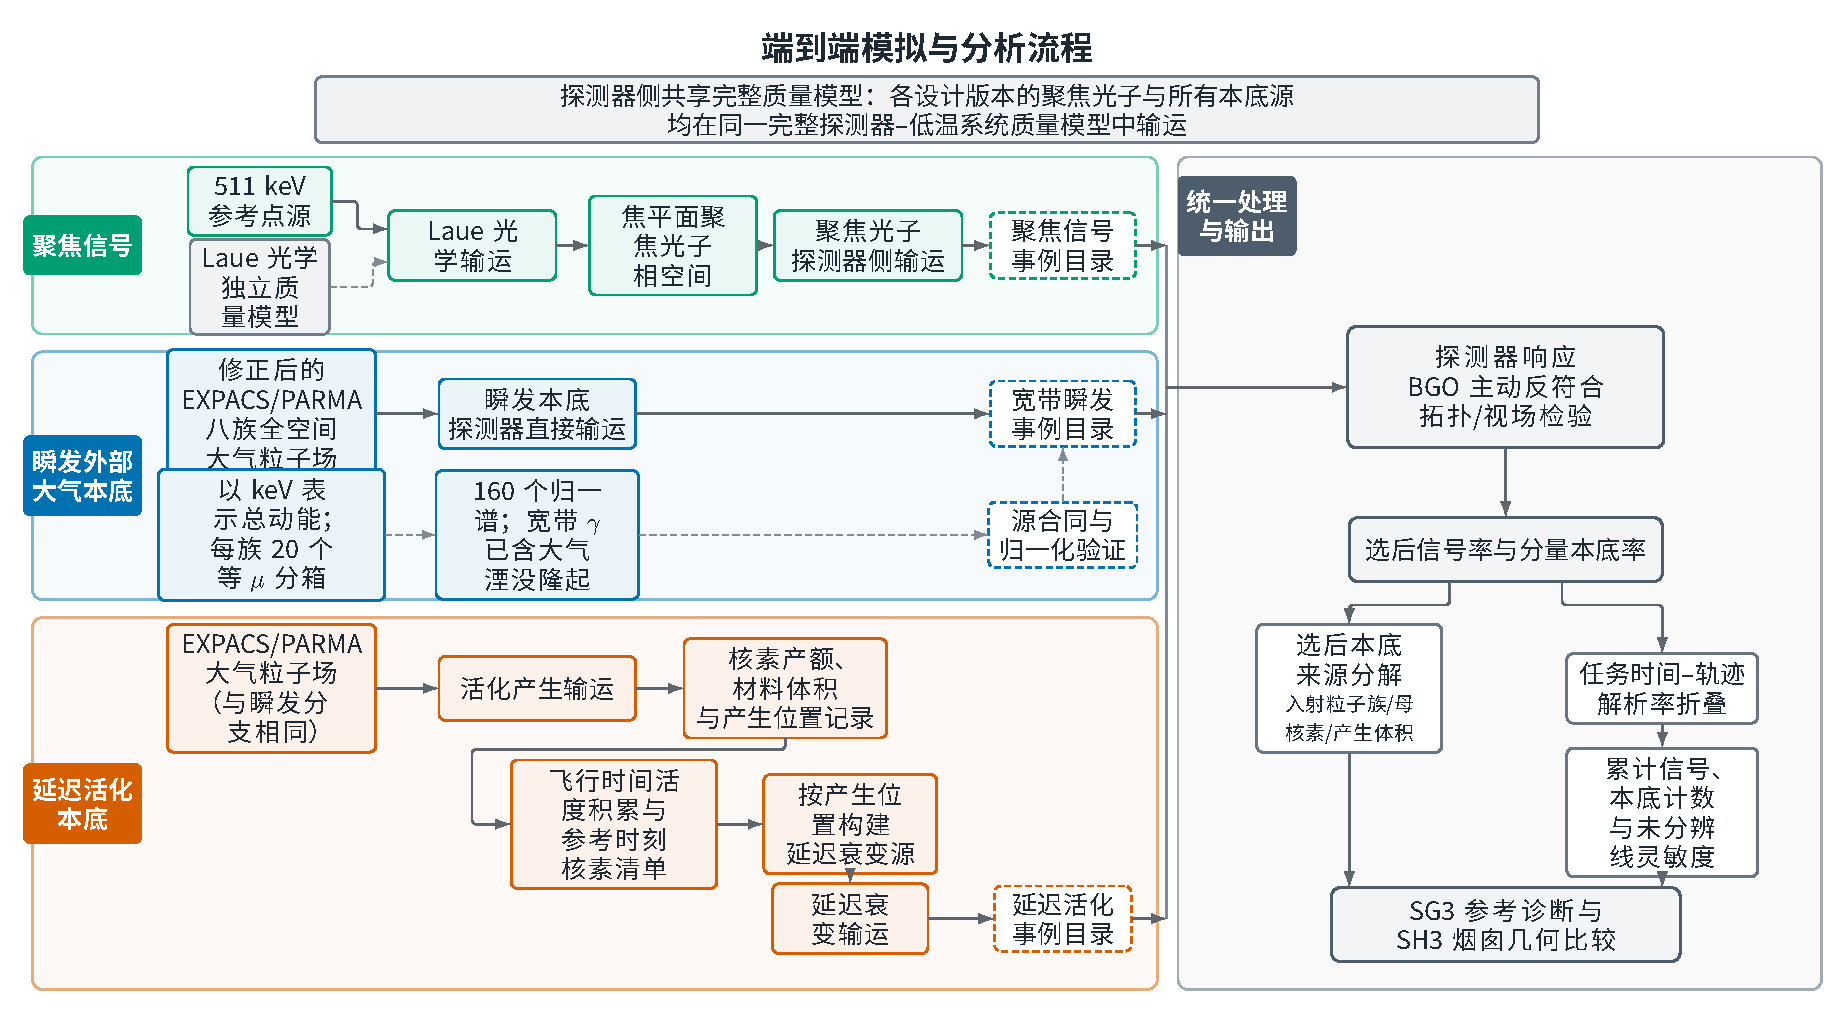
\includegraphics[width=0.94\linewidth]{figures/fig02_workflow_zh.pdf}
\captionof{figure}{端到端模拟与分析流程。聚焦信号、经正确总动能修复的八族大气场和按产生位置抽样的活化衰变分别输运，随后统一施加探测器响应、科学窗、主动 BGO 反符合及拓扑/视场选择。选后率进入来源分解和 81 节点任务折叠，用于 SG3--SH3 同口径比较。}
\label{fig:workflow}
\vspace*{\fill}
\end{landscape}

\FloatBarrier

\subsection{Laue 光学与探测器耦合信号输运}
\label{sec:optics}

本文模拟采用基于镶嵌型 Ge(111) 晶体的 Laue 透镜系统 \cite{Barriere2009Laue,Barriere2011LauePrototype}，通过光学设计实现 $10\,\mathrm{m}$ 的焦距、511 keV 单环参考响应，以及 511 keV 下 $20.1\,\mathrm{cm^2}$ 的有效面积；有效面积按
\begin{equation}
  A_{\mathrm{eff}}(E)=A_{\mathrm{inc}}\frac{N_{\mathrm{fp}}(E)}{N_{\mathrm{inc}}(E)}
  \label{eq:laue_aeff}
\end{equation}
计算，其中 $A_{\mathrm{inc}}$ 为蒙特卡洛入射采样面积，$N_{\mathrm{inc}}(E)$ 为入射光子数，$N_{\mathrm{fp}}(E)$ 为满足聚焦/焦面截取条件的光子数。
采用镶嵌晶体系统是为了在满足预期设计聚焦性能的同时便于蒙特卡洛计算；实际工程适配时也可考虑其他候选方案。

在本模拟中，laue光学分支给出聚焦性能模拟，并使聚焦信号穿过 Ge 晶体质量输运。

为此,晶体对光子的衍射概率不再作为一个效率参数叠加给光子,而是在 Geant4 应用层定义为一个离散过程 \cite{Agostinelli2003,Allison2016}。该过程按当前光子相对晶面的角偏差取衍射概率 $R(|\Delta\theta|)$,并把它转换为一个有限的等效衍射平均自由程 $\lambda_{\mathrm{diff}}$,使光子穿过晶体路径 $\ell$ 时累计的衍射概率复现该值:$1-\exp(-\ell/\lambda_{\mathrm{diff}})=R(|\Delta\theta|)$,即 $\lambda_{\mathrm{diff}}=-\,\ell/\ln[1-R(|\Delta\theta|)]$;为避免与标准光电吸收重复计数,$R$ 先按未吸收份额归一($R/(1-A)$)再转成自由程。该自由程交回 Geant4 后,衍射过程与标准电磁过程(光电吸收、康普顿散射)在同一竞争框架下各自抽样相互作用长度,由最短者决定谁先发生,而不是在晶体边界强制拦截光子。未被抽中发生衍射的光子仍按标准电磁物理继续输运,可能被吸收、散射或直接透射。

衍射概率优先由外部 XOP/CRYSTAL rocking-curve map 按角偏差插值给出:该曲线由 XOP 工具包的 CRYSTAL/diff\_pat 模块(经 xoppylib 调用,以 DABAX 晶体学数据为输入)在预处理阶段一次性离线计算 \cite{SanchezDelRio2011XOP},给出 Ge(111) 反射率/透射率/吸收随角偏差的曲线;输运过程中对晶体内每一步实时计算角偏差,在该曲线上插值取当前衍射概率,即“库离线建表、概率随输运按角取用”。mosaic 取向通过对理想 Bragg 晶面法线施加高斯角扰动实现,扰动宽度由 30 角秒 mosaic FWHM 给出;衍射发生后,出射方向按扰动后的晶面法线镜面反射,光子能量不变。这种“过程类只负责输运接口、独立模型类负责概率与方向判定”的拆分方式,借鉴了 Geant4 中已有的晶体 Bragg 反射扩展工作的思路 \cite{Guan2023BraggReflection,Reiazi2025G4BraggReflection}，扩展到我们所需能段。

这里的参考信号是一个单色 511 keV 点源；其大气层顶取整参考尺度 $\fzero=10^{-4}\phcms$（见第~\ref{sec:requirements} 节）由 INTEGRAL/IBIS 的专门紧凑源上限提供依据，而非取自某个已观测天体 \cite{DeCesare2011}。信号以 MEGAlib 远场源方式构建 \cite{Zoglauer2006}，详细构建方式见第~\ref{subsec:pointsource} 节。信号经光学分支输运并作为平行束源输入探测器质量模型；宇宙线瞬发本底与活化衰变则直接在探测器/低温系统质量模型中输运。因此，主要本底预算定义在探测器/低温系统分支上，光学分支提供输运到焦平面的信号相空间。

\subsection{源构建}
\label{sec:background}

在第~\ref{sec:optics} 节定义聚焦光学后，本文分别构建聚焦点源、瞬发大气场和延迟放射性群体。活化产生与延迟衰变输运仍是延迟链中两个独立阶段。这样在施加共同探测器响应和事例选择前，每个分量都保留自己的归一化以及“粒子族--核素--产生位置”来源关系。

\subsubsection{瞬发大气源}
\label{subsec:prompt_source}

瞬发大气粒子场由 EXPACS/PARMA 给出。PARMA3.0 是由 PHITS 大气级联计算参数化得到、
并针对陆地宇宙线测量验证过的解析模型，EXPACS 是其公开表格与软件接口
\cite{Sato2015EXPACS,Sato2016PARMA4}。底层的粒子输运物理由 PHITS 提供：一次宇宙线
与大气核作用，次级强子、轻子、光子和中子在大气柱中继续输运，最终通量按海拔、
地磁截止刚度、太阳调制、能量和方向参数化。本文中 EXPACS/PARMA 给出随粒子种类、
动能、天顶角、地理位置、海拔、截止刚度和太阳活动变化的入射微分通量，且只用于构造
外部辐射场；探测器响应、反符合、拓扑选择和任务时间计数都在下游施加。参考源定义
采用纬度 $34^\circ$、经度 $100^\circ$、海拔 $38\,\mathrm{km}$、垂直截止刚度
$R_c=11.6\,\mathrm{GV}$，以及 2025-08-31 对应的太阳条件 $W=118.3$。

瞬发源包含光子、中子、电子、正电子、质子、$\alpha$ 粒子以及正负 $\mu$ 子。对每个
粒子族，EXPACS/PARMA 微分谱被转换为 MEGAlib 远场面积源，覆盖完整天顶角范围
$\theta=0^\circ$--$180^\circ$ 和完整方位角范围 $\phi=0^\circ$--$360^\circ$。天顶角
依赖用 20 个等 $\mu$ 微分分箱表示，其中 $\mu=\cos\theta$，每箱立体角
$\Delta\Omega=0.6283185307\,\mathrm{sr}$：前 10 箱为下行粒子，后 10 箱为上行或反照
成分。瞬发输运和活化产生输运都保留这两个半球，因此源构建阶段没有丢弃上行反照
粒子。图~\ref{fig:expacs_fullsphere_flux} 给出由源定义实际采用的全空间通量场。

\begin{figure}[t]
\centering
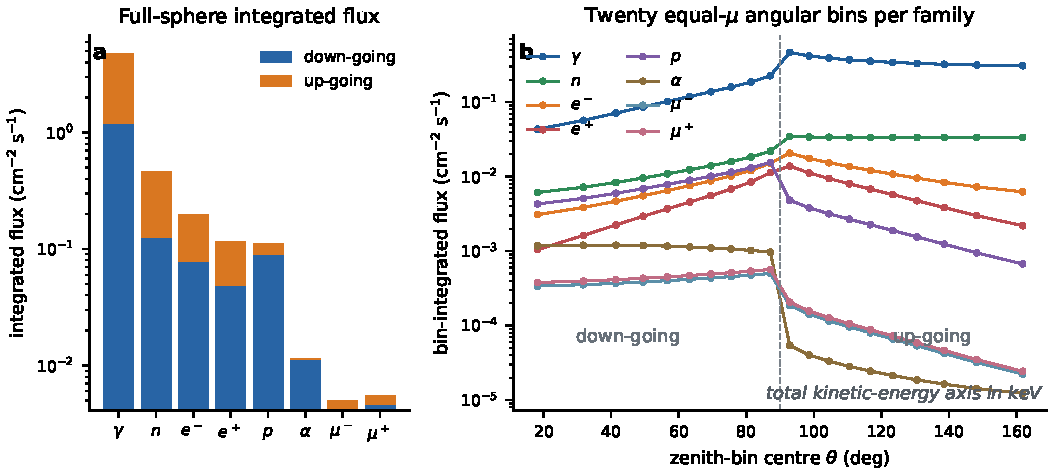
\includegraphics[width=\linewidth]{figures/fig03_corrected_kev_sources.pdf}
\caption{用于瞬发输运与活化产生的正确总动能 EXPACS/PARMA 大气场。（a）八类粒子族按上、下行半球分开的能量和立体角积分通量。（b）各远场源采用的 20 个等 $\mu$ 天顶角分箱积分通量。环境参数为纬度 $34^\circ$、经度 $100^\circ$、海拔 $38\,\mathrm{km}$、$R_c=11.6\,\mathrm{GV}$ 和 $W=118.3$。}
\label{fig:expacs_fullsphere_flux}
\end{figure}

全空间积分通量分别为 4.79966、0.462239、0.199002、0.116981、0.112301、0.0114871、0.00496893 和 $0.00557001\,\mathrm{cm^{-2}\,s^{-1}}$，依次对应 $\gamma$、$n$、$e^-$、$e^+$、$p$、$\alpha$、$\mu^-$ 和 $\mu^+$。每一族均采用 20 个等 $\mu$ 分箱和半径 60 cm 的远场起始球。少数族可以增加 Monte Carlo 抽样，但每族始终保留独立输运曝光
\begin{equation}
  r_{\mathrm{event},j}=\left(\sum_i \mathcal{T}_{ij}\right)^{-1},
\end{equation}
其中 $\mathcal{T}_{ij}$ 为粒子族 $j$ 的第 $i$ 个子样本曝光。因此增加抽样只改变统计方差，不改变物理期望率。

送入 Cosima 的能量轴为 keV 单位的总动能：非 $\alpha$ 粒子采用 $E_{\mathrm{tot,keV}}=1000E_{\mathrm{MeV}}$，$\alpha$ 粒子采用 $E_{\mathrm{tot,keV}}=4\times1000E_{\mathrm{MeV/nucleon}}$。保留源包共有 160 张归一化能谱（每族 20 张）和 24 张几何专用源卡；其数值积分范围为 $0.999999999991$--$1.000000000006$，480 个能谱引用全部指向正确能量约定。

角度归一与能谱归一被有意拆开。若 $I_j(E,\mu)$ 表示粒子族 $j$ 的 EXPACS/PARMA 微分强度，则等 $\mu$ 分箱 $m$ 承载的通量为
\begin{equation}
 \Phi_{j,m}=2\pi\int_{\mu_m}^{\mu_{m+1}}\!\mathrm d\mu
             \int I_j(E,\mu)\,\mathrm dE,
 \qquad \Delta\mu=0.1,
 \label{eq:source_bin_flux_zh}
\end{equation}
故每箱立体角为 $\Delta\Omega=2\pi\Delta\mu=0.62831853\,\mathrm{sr}$。前 10 箱覆盖下行半球，后 10 箱覆盖上行或反照半球，两者方位角均完整。每箱内部能谱归一为一，物理幅度由 $\Phi_{j,m}$ 承载；这样不会把能谱表的归一误当作粒子通量。

八族使用同一个半径 60 cm 的包围源球和同一方向约定。给定抽样方向后，起点取自在该方向上的投影圆盘，动量指向质量模型内部。因此几何率因子是投影面积 $\pi R^2$，而不是球面面积 $4\pi R^2$。这里的“全空间”表示入射立体角完整，并不表示在球壳任意位置均匀向内发射。该区别同时影响瞬发输运和活化产生；若面积语义错误，所有率与活度都会按同一因子线性偏移。

正确能量约定在任何输运归一之前施加。电子、正电子、光子、核子和 $\mu$ 子的表格动能乘 $10^3$，把 MeV 转为 keV；$\alpha$ 表格以每核子 MeV 给出，因此还需乘质量数四。若对 $\alpha$ 与其他七族使用同一个转换式，其总动能会再少四倍；若把表中 MeV 数值直接解释为 keV，则全部粒子族的能量轴会低三个数量级。当前源合同显式记录两种情况，不依赖隐含单位约定。

源包检查覆盖真正进入物理归一的量：每个粒子族有 20 张有限、非负能谱；每张能谱的数值积分均在上述精度内为一；全部源卡引用都能解析到正确 keV 能谱集；源卡几何头还必须与实际输运质量模型一致。瞬发输入和活化产生输入共享大气场定义，但仍是两个独立计算，因而活化产物不会既作为即时探测器事例、又作为后续衰变重复计数。

这一构建也限定了能够从光子分量推断的物理量。$4.79966\,\mathrm{cm^{-2}\,s^{-1}}$ 是保留能区内的宽带全空间光子积分通量；能谱同时含有湮没增强及其相邻连续谱。科学窗率必须通过该宽带分量的输运和响应卷积获得，而不是把另行拟合的大气线流量乘探测效率。这样既避免双计数，也不对源合同层面不可分辨的光子作人为拆分。

\subsubsection{宽带大气光子分量}
\label{subsec:atm511_source_zh}

修复后的大气光子表作为一个宽带 $\gamma$ 分量处理。保留谱同时含有 511 keV 附近的湮没特征及周围连续谱，因此再加入独立大气单能源会重复计数同一物理成分。该 $\gamma$ 分量与其他七族一样使用 20 分箱全空间几何、逐族曝光归一、共同探测器响应及随轨迹变化的粒子族尺度。

该约定仍然严格区分天体信号和局地大气光子：科学信号是聚焦的轴上 EventList；大气光子只从宽带瞬发目录进入，并在选择后通过入射粒子族标签分解。

\subsubsection{延迟活化源}
\label{subsec:delayed_source}

延迟源来自独立的活化产生输运。活化记录不作为即时本底计数，而是保存每个放射性产物的核素、材料体积、入射粒子族和产生位置；基态半衰期对照 NUBASE2020 校验 \cite{Kondev2021NUBASE}。对核素 $k$，
\begin{equation}
  A_k(t_{\mathrm{flight}})=P_k\left[1-\exp(-\lambda_k t_{\mathrm{flight}})\right],
  \qquad \lambda_k=\frac{\ln2}{t_{1/2,k}},
\end{equation}
其中 $P_k$ 为产生率，参考状态取 $t_{\mathrm{flight}}=15\,\mathrm{d}$。全八族第 15 天活度为 SG3 的 $1352.29749\,\mathrm{Bq}$ 和 SH3 的 $211.387433\,\mathrm{Bq}$。

仅有聚合清单不足以构建该源。活化产生计算还在放射性产物形成时保留坐标记录，并按材料体积、核素和激发态将第 15 天群体与这些记录匹配。所得源描述按入射粒子族、材料类别、产生体积和坐标组织。这些量属于源构建而非探测器计数；只有当延迟粒子从共同几何中的记录位置发射后，才施加衰减、衰变输运、探测器响应和事例选择。

保留位置是必要的，因为下游衰减、主动屏蔽概率和拓扑取决于核素产生地点。产生记录按体积、核素、激发态和坐标匹配后再进行衰变输运。入射族 $a$、$b$ 的活度归一材料分布可用
\begin{equation}
  D_{\mathrm{TV}}(a,b)=\frac12\sum_c|f_{a,c}-f_{b,c}|
\end{equation}
比较，其中 $f_{a,c}$ 是族 $a$ 在材料类别 $c$ 中的活度比例。只保留体积积分活度会抹掉决定最终科学窗本底的“粒子族--材料--核素--坐标”相关性。

设产生表第 $j$ 行的活度权重为 $w_j$、总活度为 $A=\sum_jw_j$。以 $p_j=w_j/A$ 有放回抽取 $M$ 个产生位置并为每个点赋予 $A/M$ 通量，则
\begin{equation}
  \mathbb{E}\!\left[N_j\frac{A}{M}\right]=Mp_j\frac{A}{M}=w_j,
\end{equation}
所以采样源对空间加权分布无偏并守恒总活度。现行每族目录均输运 $10^6$ 个延迟衰变；SH3 共含 $8\times10^6$ 个延迟触发，完整科学窗、BGO 和拓扑选择后保留 111 条记录。其第 15 天分族活度依次为 $\alpha$ 34.2836、$e^-$ 0.2663、$e^+$ 0.6754、$\gamma$ 2.0320、$\mu^-$ 0.0684、$\mu^+$ 0.0040、$n$ 68.5316 和 $p$ 105.5262 Bq。

表~\ref{tab:background_source_model} 汇总两个几何共同采用的源层级；探测器响应、反符合与拓扑选择均在下游施加。

\begin{table}[t]
\centering
\caption{SG3 与 SH3 共同采用的源层级。表中只定义源构建，探测器响应和选择在下游施加。}
\label{tab:background_source_model}
\footnotesize
\begin{tabular}{p{0.21\linewidth}p{0.34\linewidth}p{0.37\linewidth}}
\toprule
层级 & 物理作用 & 当前实现 \\
\midrule
正确能量大气场 & 瞬发探测器命中和活化产生 & 八族、每族 20 个等 $\mu$ 分箱、全空间、60 cm 起始半径；总动能以 keV 输入。 \\
宽带 $\gamma$ & 包含湮没特征的大气光子 & 单一保留宽带分量，不叠加独立大气单能归一。 \\
活化产生 & 粒子族--核素--体积--位置历史 & 使用同一正确能量大气场，并采用 NUBASE 校验的基态衰变数据。 \\
第 15 天放射性群体 & 延迟输运采用的飞行活度 & SG3：$1352.29749\,\mathrm{Bq}$；SH3：$211.387433\,\mathrm{Bq}$。 \\
产生位置衰变 & 从实际记录材料坐标发射延迟粒子 & 每族 $10^6$ 次衰变；每个几何含八个独立归一族目录。 \\
\bottomrule
\end{tabular}
\end{table}

最终延迟事例仍保留母核身份与精确产生体积。SG3 的主导组包括 L2 铜支撑环和 50 mK 混合室板内的 $^{62}$Cu；SH3 最大组是 L5 铜环中的 $^{62}$Cu，其次为 TES 热沉环中的 $^{62}$Cu，W 框和 Al 壳组更小。真正驱动第~\ref{subsec:reference_background_results_zh}~小节几何解释的是这些选后来源，而非未筛选总清单。

\subsubsection{参考点源构建}
\label{subsec:pointsource}

聚焦信号流由一个单色 511 keV 参考点源定义。其通量尺度不取自某个特定天体，而是
参照 INTEGRAL/IBIS 的专门紧凑源上限取整为大气层顶
$\fzero=10^{-4}\phcms$（见第~\ref{sec:requirements} 节）\cite{DeCesare2011}。

由于此类源位于天文距离处，它被建模为理想轴上点源：在光学计算中，它是平行于光轴入射并在式~(\ref{eq:laue_aeff}) 的入射孔径 $A_{\mathrm{inc}}$ 上均匀抽样的单色 $511\keV$ 远场光束。源本身不赋予有限角尺寸；焦面角结构完全由 30 角秒 mosaic 展宽、XOP/CRYSTAL 摇摆曲线和 10 m 聚焦几何产生，因此接受光子形成有限光斑而非单一射线。三个独立光学样本共含 $1.5\times10^5$ 个入射光子，得到 37,256 个衍射焦面穿越，其中 37,194 个落入半径 $1.898\,\mathrm{cm}$ 的 Be 入射窗；光斑半径为 $r_{90}=1.03\,\mathrm{cm}$、$r_{99}=1.25\,\mathrm{cm}$。每个接受穿越所记录的位置和方向构成两个几何共用的探测器侧 EventList。

探测器入口聚焦率为
\begin{equation}
  R_{\mathrm{fp}}=F_{\mathrm{TOA}}\,\aeff(511\keV)\,T_{\mathrm{atm},45}.
\end{equation}
等价地，生成光学样本代表曝光 $N_{\mathrm{fp}}/[F_{\mathrm{TOA}}\aeff T_{\mathrm{atm},45}]$，每个 EventList 条目以该曝光的倒数作为物理率权重。这样可把探测器侧接受度与大气层顶通量归一分开，并确保后者只施加一次。光学计算只包含源光子；全部本底仍只从上文定义的大气流和延迟活化流进入。
第 15 天 $T_{\mathrm{atm},45}=0.652034$。SG3 有 28,612 条记录落入测量科学窗，28,006 条通过最终拓扑选择，得到 $A_{\mathrm{eff}}=15.12324\pm0.04492\,\mathrm{cm^2}$；SH3 相应为 28,434、27,936 条及 $15.08544\pm0.04503\,\mathrm{cm^2}$。施加大气透过和第 15 天偶然符合存活后，在 $F_{\mathrm{TOA}}=10^{-4}\phcms$ 下两者信号率分别为 $9.5362\times10^{-4}$ 和 $9.7904\times10^{-4}\cps$。因此烟囱只改变 $0.25\%$ 的选后面积，却显著改变本底环境。

上文引用的有效面积为轴上值，代表最佳指向情形。点源偏离光轴、或飞行中的残余姿态抖动，
会通过 Laue 透镜有限的角接受（视场）降低并移动聚焦响应
\cite{Barriere2009Laue,Weidenspointner2006MAX}；这一离轴依赖作为对信号有效面积的指向
系统学处理，而不改变轴上参考构建。当前侧入射响应是固定 $45^\circ$ 仰角参考，
并非已完成的银心低仰角模拟。

\subsection{由本底来源驱动的几何设计与统计方法}
\label{subsec:comparison_hierarchy_zh}

设计从真正进入科学窗的事例出发。SG3 的最终瞬发事例按入射族分组，延迟事例按入射族、母核素、产生材料、体积和坐标分组；这一分量优先逻辑与 COSI 和 DIXE 的细致本底研究一致 \cite{Gallego2025Balloon,Tian2026DIXE}。结果显示 SG3 的多级冷端区域正投影在焦面上方，因此 SH3 将 TES 横向平移到侧烟囱，同时保持光学接受度，并用主动 BGO 环绕新焦面。

Cosima 沉积先按 TES 像素聚合，再独立施加 $\Delta E_{\mathrm{FWHM}}=0.420\keV$（$\sigma=0.17836\keV$）的高斯响应。低于 $0.300\keV$ 的测量命中被移除，其余命中在科学窗、BGO 与拓扑判断前求和。两个几何采用完全相同的响应约定。

对流 $k$ 和阶段 $j$，物理率、Monte Carlo 标准误差和有效支撑为
\begin{equation}
  \widehat R_{k,j}=\sum_{i\in(k,j)}w_i,\qquad
  \sigma_{k,j}=\left(\sum_{i\in(k,j)}w_i^2\right)^{1/2},\qquad
  N_{\mathrm{eff},k,j}=\frac{\widehat R_{k,j}^2}{\sigma_{k,j}^2}.
  \label{eq:weighted_rate_stats_zh}
\end{equation}
记录数表示输运支撑，带权率表示物理本底。本文还保留阶段存活率 $q_{k,j}=\widehat R_{k,j}/\widehat R_{k,\mathrm{window}}$ 和最终分量占比 $f_k=\widehat R_{k,\mathrm{final}}/\sum_b\widehat R_{b,\mathrm{final}}$；当各分量曝光不同时，少量输运记录仍可能承载重要物理率。

同一独立归一输运分量内的事例权重恒定，因此双侧 95\% Garwood 泊松计数区间乘以单事例权重即可得到精确率区间。具有明确曝光但零条选后记录的分量给出率上限，而不是“物理本底为零”；聚焦信号接受度则按二项分布用相应精确区间检验。这些逐分量边界只诊断有限输运支撑，并非联合覆盖带，也不包括辐射场、截面、标定或指向系统学。主任务不确定度另用 delta 方法传播本底输运、公共时间、选后面积和偶然符合探针项。

对轨迹时间箱 $\ell$、活时间比例 $L_\ell$ 与时长 $\Delta t_\ell$，
\begin{equation}
 N_s(T)=\sum_{\ell\le T}S_\ell L_\ell\Delta t_\ell,\qquad
 N_b(T)=\sum_{\ell\le T}B_\ell L_\ell\Delta t_\ell.
 \label{eq:cumulative_counts_zh}
\end{equation}
本文同时报告高斯计数指标 $Z_G=N_s/\sqrt{N_b}$ 与 Asimov 形式
\begin{equation}
 Z_A=\sqrt{2\left[(N_s+N_b)\ln\left(1+\frac{N_s}{N_b}\right)-N_s\right]}.
\end{equation}
最小流量由同一信号核求解 $Z=3$ 或 5，使任务比较保持统一统计与物理归一。

\subsection{探测器事例选择与 veto 定义}
\label{sec:selection}


聚焦信号、瞬发大气和延迟活化目录被放在一条显式时间轴上；随后对两个几何施加相同的测量科学窗、主动 BGO 反符合与拓扑/视场定义。宽带瞬发 $\gamma$ 已包含大气湮没特征，因此率预算中没有额外大气线目录。

\subsubsection{时间轴与率归一}

每条流的记录具有率权重 $r_{km}$，总率为 $R_k=\sum_mr_{km}$。对参考区间 $T$，各流独立抽取
\begin{equation}
 N_k\sim\mathrm{Pois}(R_kT),
\end{equation}
再按 $r_{km}/R_k$ 选取记录、在 $[0,T]$ 内赋予均匀时刻、合并并排序。间隔不超过 $\tau=1\,\mu\mathrm{s}$ 的记录组成一个符合组。第 0、5、10、15 和 20 天各采用 $2\times10^5$ s 锚点检验。图~\ref{fig:s33_poisson} 比较公共时间率与独立归一直接率，图~\ref{fig:s33_spec_norm} 给出两个几何的带权预 veto 能谱。第 15 天公共时间率与直接率之比为 SG3 的 0.9665 和 SH3 的 1.0172，与有限锚点计数相符；信号偶然符合存活因子分别为 0.967071 和 0.995341。

\begin{figure}[t]
\centering
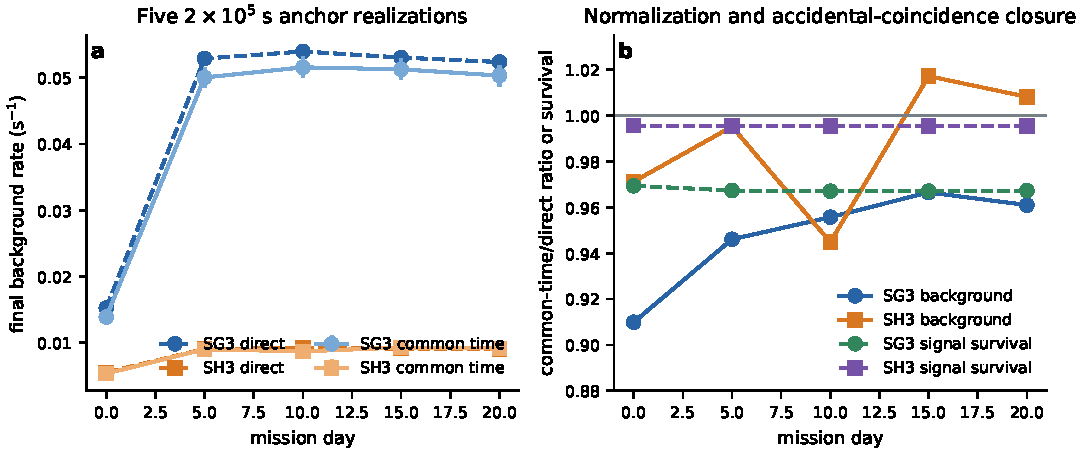
\includegraphics[width=\linewidth]{figures/fig04_common_time_normalization.pdf}
\caption{五个任务锚点的公共时间归一。（a）SG3 与 SH3 的无符合直接最终本底率和 $2\times10^5$ s 公共时间率；误差棒为锚点实现的泊松标准误差。（b）公共时间/直接本底率比及聚焦信号偶然符合存活因子。所有锚点采用同一 $1\,\mu\mathrm{s}$ 分组约定。}
\label{fig:s33_poisson}
\end{figure}

\begin{figure}[t]
\centering
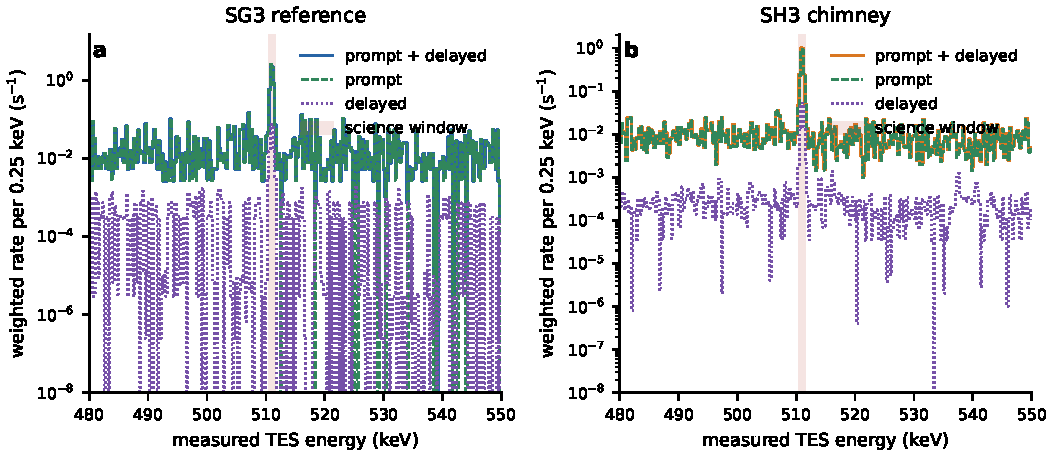
\includegraphics[width=0.82\linewidth]{figures/fig05_pre_veto_spectra.pdf}
\caption{主动 veto 前经响应卷积的带权瞬发加延迟能谱：（a）SG3 参考几何；（b）SH3 烟囱几何。阴影带为 $510.58$--$511.42\keV$ 科学窗；绝对 cut-flow 率见表~\ref{tab:phase2_cutflow} 与表~\ref{tab:optimized_cutflow_zh}。}
\label{fig:s33_spec_norm}
\end{figure}

任务折叠在每个轨迹箱使用公共时间期望
\begin{equation}
 L_\ell=\exp\!\left\{-\tau\left[R^{\mathrm{occ}}_{\mathrm{prompt},\ell}+R^{\mathrm{occ}}_{\mathrm{delayed},\ell}\right]\right\}.
 \label{eq:atm511_live_factor_zh}
\end{equation}
弱聚焦源不进入指数；更亮源应用应显式加入其占有率。大气与活化率按任务日变化，符合分组发生在微秒尺度，因此每个时间箱视为平稳叠加。五个显式锚点验证符合构建，81 节点折叠使用其期望，而不在每个时间箱重新抽取随机实现。

\subsubsection{主动反符合门}

第一层为主动 BGO 反符合。对符合组 $c$，
\begin{equation}
 E_{\mathrm{TES}}^{(c)}=\sum_{j\in c}E_{\mathrm{TES},j},\qquad
 E_{\mathrm{sh}}^{(c)}=\sum_{j\in c}E_{\mathrm{sh},j}.
\end{equation}
当
\begin{equation}
 \wii=[510.58,511.42]\keV
\end{equation}
且
\begin{equation}
 E_{\mathrm{sh}}^{(c)}<E_{\mathrm{veto}},\qquad E_{\mathrm{veto}}=50\keV
\end{equation}
时通过主动屏蔽。SG3 直接目录中，瞬发样本由 1083 条、$5.79018\cps$ 降至 7 条、$1.87041\times10^{-2}\cps$；延迟样本由 1295 条、$0.169494\cps$ 降至 436 条、$4.34116\times10^{-2}\cps$。测量窗内 28,612 条 SG3 信号记录全部通过主动反符合。图~\ref{fig:s33_spec_anti} 显示 SH3 BGO 的更强抑制。

\begin{figure}[t]
\centering
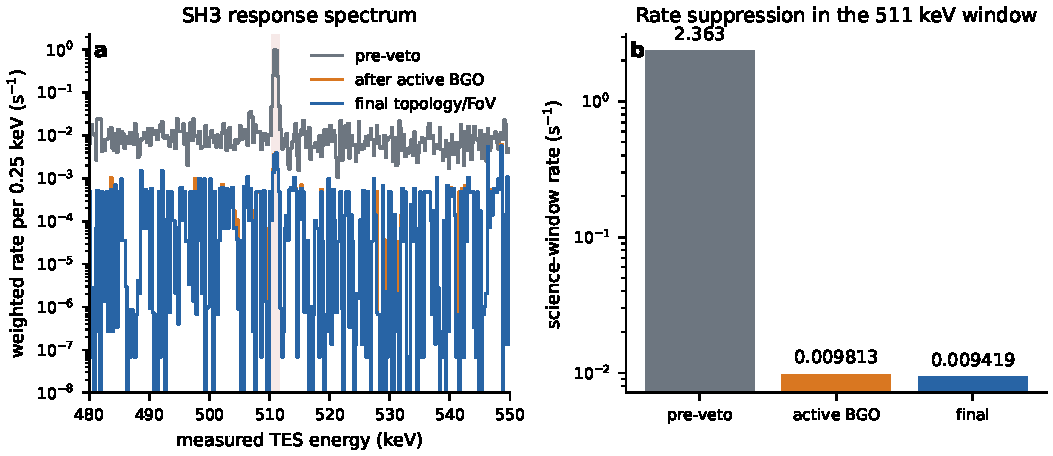
\includegraphics[width=0.82\linewidth]{figures/fig06_bgo_veto_spectrum.pdf}
\caption{SH3 烟囱几何的主动 BGO 抑制。（a）480--550 keV 带中 veto 前、BGO 后和最终拓扑/视场后的带权能谱。（b）科学窗对应率；主动 BGO 将直接本底由 $2.36263$ 降至 $9.8133\times10^{-3}\cps$。}
\label{fig:s33_spec_anti}
\end{figure}本文给出的流量阈值适用于经探测器响应后本征宽度相对该线窗仍较小的谱线；若源线明显展宽，须将源线型与响应卷积并重新优化窗宽。

\subsubsection{康普顿拓扑与视场一致性}

第二层对通过主动屏蔽的 TES 命中施加基于康普顿运动学的拓扑与视场一致性检验，其物理基础是康普顿相机的成锥重建~\cite{Zoglauer2006}。能量为 $E_0$ 的入射光子在第一作用点 $\mathbf r_1$ 发生康普顿散射、沉积能量 $E_1$，散射光子携带能量 $E_{\mathrm{sc}}=E_0-E_1$ 前进至下一作用点 $\mathbf r_2$，散射角 $\theta_C$ 由
\begin{equation}
  \cos\theta_C =
  1 - m_ec^2\left(\frac{1}{E_{\mathrm{sc}}}
  - \frac{1}{E_1+E_{\mathrm{sc}}}\right)
\end{equation}
给出。已知散射光子的飞行方向 $\hat{\mathbf u}_{12}=(\mathbf r_2-\mathbf r_1)/|\mathbf r_2-\mathbf r_1|$ 后，源的方位被约束在以 $\mathbf r_1$ 为顶点、$-\hat{\mathbf u}_{12}$ 为轴、半张角 $\theta_C$ 的重建圆锥面上，其在天球上的投影即事例圆。这里把第一散射锥用于孔径一致性检验：当锥面与侧入射 Be 窗圆盘（半径 $1.898\,\mathrm{cm}$）相交，即保留该事例，亦即其重建来向与穿过入射孔径相容。

由于单个 TES 像素（$1.5\times1.5\times3.0\,\mathrm{mm}$）的内部作用位置不可分辨，本文不以像素质心单点、而以 $8+1=9$ 个代表点（八个像素角点与质心）表征每个命中，从而把亚像素位置不确定性显式带入几何重建。据此，一个双命中事例在给定散射次序下枚举 $9\times9=81$ 组首/次作用点组合，对每组构造一条重建圆锥（锥面以 24 个方位角离散采样后延拓至 Be 窗平面，并同时以采样点与相邻线段判定与窗盘的相交）；只要这 81 条轨迹中存在任一条使锥面与 Be 窗盘相交，即判该次序视场相容。这是一个刻意从宽的一致性判据：只要像素内部存在与穿过入射孔径相容的作用位置假设即予保留。因此该层保留了约 $95\%$ 的窗内多命中事例、仅削减约 $10$--$14\%$ 的本底，与其宽松一致性 veto、而非成像重建的定位一致。

据此对三类事例分别处理。单像素事例作为量热线候选保留；双命中同时检验两种作用次序和代表性亚像素位置，任一次序相容即保留；三至六命中枚举全部次序，并以康普顿序列残差
\begin{equation}
 Q=\sum_{i=1}^{n-2}\left(\cos\theta_{C,i}-\hat{\mathbf u}_{i-1,i}\!\cdot\!\hat{\mathbf u}_{i,i+1}\right)^2
\end{equation}
排序，最优次序再接受同一锥--孔径检验。SG3 拓扑层保留 443 条主动 veto 后本底中的 400 条，带权率存活 $87.41\%$，并保留 28,612 条信号中的 28,006 条；SH3 相应保留 134 条中的 123 条本底，带权率存活 $95.98\%$，以及 28,434 条中的 27,936 条信号。图~\ref{fig:s33_compton_mult} 按 TES 命中多重度分解这些样本。

\begin{figure}[t]
\centering
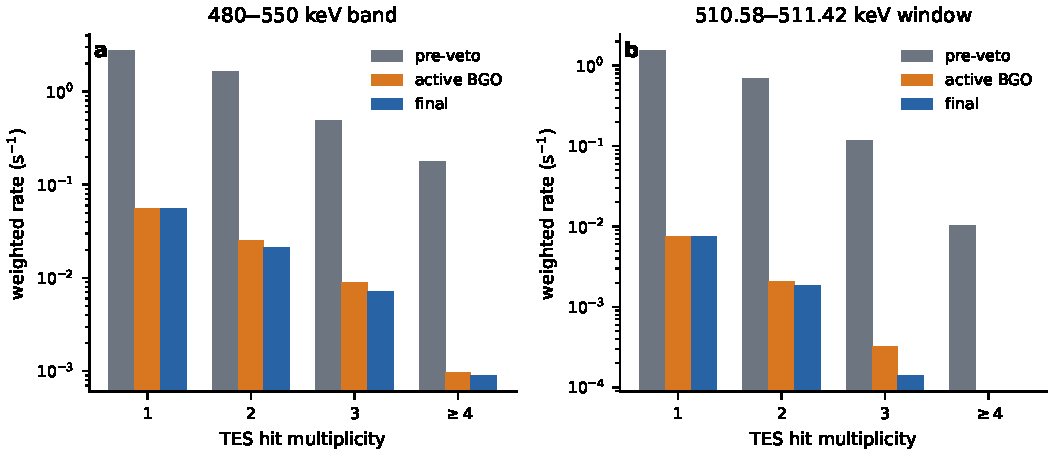
\includegraphics[width=\linewidth]{figures/fig07_hit_multiplicity.pdf}
\caption{SH3 带权本底率按 TES 命中多重度的分解，依次给出 veto 前、主动 BGO 后及拓扑/视场后：（a）480--550 keV 宽带；（b）$510.58$--$511.42\keV$ 科学窗。多命中事例在康普顿锥与入射孔径相容时保留。}
\label{fig:s33_compton_mult}
\end{figure}

未重建类仍计入率核算，但不标记为视场一致候选。实测多重度分布表明，主动 BGO 提供主要率压低，拓扑只移除较小残余，同时保留聚焦的多命中信号。表~\ref{tab:phase2_cutflow} 给出 SG3 在直接、无符合归一上的参考 cut-flow；任务率由公共时间折叠得到。

\begin{table}[t]
\centering
\caption{SG3 参考几何科学窗 cut-flow。本底为直接无符合记录数/率；信号为共同 37,194 光子焦面样本的记录数/有效面积。}
\label{tab:phase2_cutflow}
\footnotesize
\begin{tabular}{lccc}
\toprule
计算流 & 预 veto & 主动 veto 后 & 最终拓扑/视场后 \\
\midrule
瞬发本底 & 1083 / $5.79018\cps$ & 7 / $1.87041\times10^{-2}\cps$ & 6 / $1.60321\times10^{-2}\cps$ \\
延迟活化 & 1295 / $0.169494\cps$ & 436 / $4.34116\times10^{-2}\cps$ & 394 / $3.82661\times10^{-2}\cps$ \\
总本底 & 2378 / $5.95968\cps$ & 443 / $6.21157\times10^{-2}\cps$ & 400 / $5.42982\times10^{-2}\cps$ \\
聚焦信号 & 28612 / $15.45048\,\mathrm{cm^2}$ & 28612 / $15.45048\,\mathrm{cm^2}$ & 28006 / $15.12324\,\mathrm{cm^2}$ \\
\bottomrule
\end{tabular}
\end{table}

保留的命中级目录提供了无需新增输运的内部检验：每个选后事例都保存测量命中能量、TES 层、像素位置和多重度。由这些字段重算宽带及科学窗，可逐项复现表中阶段计数，并确认拓扑层位于主动 BGO 判断之后。

\subsection{任务时间轨迹与解析率折叠}
\label{sec:mission_time_fold}

MeV 气球观测由本底主导：大气次级粒子和宇宙线诱发活化共同设定率底，且二者都随飞行环境变化 \cite{Gallego2025Balloon,Kierans2017}。固定几何的探测器耦合 Monte Carlo 已在共同响应、veto 和能窗下给出第 15 天选后信号与本底率，但这些率只描述单一经纬度和海拔。多日浮空期间，残余大气深度、地磁截止和活化库存均会演化，因此不能用恒定率把第 15 天快照直接外推。本文把参考率映射到连续 20 d 性能曲线，并保留显式公共时间锚点作为时间轴构建的独立检验。

所采用的轨迹是\emph{合成参考剖面}，既非气球遥测，也非源可见性时间表。它包含第 0--20 天的 81 个节点，间隔 0.25 d，并围绕海拔 38.75 km、纬度 $34^\circ$ 和经度 $100^\circ$ 作温和中纬度浮空变化。保留海拔是因为残余大气深度变化同时影响驱动瞬发本底与活化的粒子谱，以及乘在聚焦信号上的 511 keV 大气透过率；经纬度只提供受控的地磁环境参考调制，不编码地球遮挡、重指向损失或某一具名源的可见性。因此，该折叠给出参考曝光灵敏度，而非某次具体发射任务的预报。

折叠由五个彼此分离的物理层组成。第一，单色点源率为
\begin{equation}
 R_{\mathrm{sig}}(t)=F_{511}A_{\mathrm{eff}}T_{\mathrm{atm},511}(t)\varepsilon_{\mathrm{det}},
 \label{eq:mission_signal_zh}
\end{equation}
其中固定 $45^\circ$ 斜程透过率 $T_{\mathrm{atm},511}(t)=\exp[-\mu_{\mathrm{air}}X(t)/\cos45^\circ]$，且 $T_{15,45}=0.652034$。第二，选后瞬发率为
\begin{equation}
 R_{\mathrm{prompt},j}(t)=\sum_b\Phi_b(t)K_{j,b},
 \label{eq:prompt_source_response_zh}
\end{equation}
八族通量 $\Phi_b(t)$ 各有自己的 81 节点尺度，$K_{j,b}$ 由几何专用探测器目录固定；保留宽带 $\gamma$ 的湮没特征已包含在该求和中。

第三，对入射族 $a$ 和放射性母核 $k$，活化产生率为
\begin{equation}
 P_{a,k}(t)=\Phi_a(t)Y_{a,k},
 \label{eq:activation_production_zh}
\end{equation}
并采用相应几何的 SG3 或 SH3 第 15 天清单。第四，库存按
\begin{equation}
 N_{a,k}(t+\Delta t)=N_{a,k}(t)e^{-\lambda_k\Delta t}+\frac{P_{a,k}(t)}{\lambda_k}\left(1-e^{-\lambda_k\Delta t}\right),\qquad
 A_{a,k}(t)=\lambda_kN_{a,k}(t)
 \label{eq:delayed_inventory_zh}
\end{equation}
推进。第五，选后延迟率为
\begin{equation}
 R_{\mathrm{delayed},j}(t)=\sum_a\sum_kA_{a,k}(t)\varepsilon_{j,a,k}.
 \label{eq:delayed_selected_zh}
\end{equation}
这些方程把天体衰减、局地瞬发调制、活化产生和放射性衰变保持为不同物理步骤。

第 0、5、10、15 和 20 天的公共时间锚点各为 $2\times10^5$ s，用于检验从直接目录到轨迹时间轴的映射。最终计算在 81 个节点施加相应分族尺度和库存演化，再用式~\eqref{eq:cumulative_counts_zh} 计算累计计数。SG3 与 SH3 因而共享源、响应、选择、计时和信号归一。

五个锚点给出定量闭合检验，而不只是曲线的视觉一致。第 0、5、10、15 和 20 天，SG3 公共时间/直接本底率比分别为 0.9099、0.9461、0.9557、0.9665 和 0.9610；SH3 相应为 0.9712、0.9952、0.9448、1.0172 和 1.0082。相对一的偏离与每个 $2\times10^5$ s 实现中有限的最终科学窗计数相符：SG3 为 293--1048 条，SH3 为 1071--1856 条。本文不使用这些比值拟合经验修正；81 节点折叠采用泊松期望，锚点只检验显式事例分组能否在计数支撑内收敛到该期望。

同一组锚点还独立检验弱聚焦事例的偶然损失。信号存活因子在 SG3 中为 0.96705--0.96937，在 SH3 中为 0.99534--0.99564；第 15 天分别为 0.967071 和 0.995341。SH3 的较高存活来自较低探测器占有率，而不是信号选择改变。该因子在共同 37,194 光子接受度计算之后相乘，从而把几何接受度、大气透过和随机符合损失保留为三个独立可审计因子。

在每个轨迹节点，八类入射族各自的瞬发响应系数固定，只改变外部场尺度。延迟计算则不同：先按粒子族缩放产生率，再用各母核半衰期推进库存，最后才施加几何专用的选后衰变效率。若只对第 15 天延迟总率乘一个统一尺度，就会抹掉短寿命与长寿命分量的差别，也无法复现任务曲线早期的增长。因此式~\eqref{eq:delayed_inventory_zh} 对每个保留的“粒子族--母核”分量在全部 81 节点分别求值。

阈值到达时间从同一累计信号与本底核得到，只在相邻轨迹节点间插值。高斯 $3\sigma$ 流量阈值的统计误差通过 delta 方法合并本底输运、公共时间、选后面积和偶然符合探针项；相对 $1\sigma$ 值为 SG3 的 7.42\% 和 SH3 的 9.36\%。SH3 中选后本底本身的相对不确定度为 18.67\%，在本底主导流量阈值中约以一半权重进入。这些量描述 Monte Carlo 与公共时间支撑，不代替辐射场、截面、标定或指向系统学。

\section{结果}
\label{sec:results}

\subsection{511 keV 线窗本底由什么决定？}
\label{subsec:reference_background_results_zh}

SG3 参考目录给出选后事例诊断。在 $510.58$--$511.42\keV$ 科学窗内，直接无符合选择保留 6 条瞬发和 394 条延迟记录，对应 $1.60321\times10^{-2}$ 与 $3.82661\times10^{-2}\cps$；总直接率为 $5.42982\times10^{-2}\cps$，独立实现的第 15 天公共时间率为 $5.12802\times10^{-2}\cps$。表~\ref{tab:reference_background_budget_zh} 按入射族分解直接率。

\begin{table}[t]
\centering
\caption{SG3 科学窗最终直接本底。不同独立归一粒子族具有不同事例权重，因此同时列出记录数与率。}
\label{tab:reference_background_budget_zh}
\footnotesize
\begin{tabular}{lrrrp{0.27\linewidth}}
\toprule
分量 & 记录数 & 率 / $\cps$ & 总本底 / \% & 选后来源 \\
\midrule
瞬发 $\gamma$ & 6 & $1.60321\times10^{-2}$ & 29.526 & 宽带大气光子 \\
延迟 $\alpha$ & 26 & $7.47607\times10^{-3}$ & 13.769 & 近场活化材料 \\
延迟 $e^-$ & 38 & $2.53793\times10^{-5}$ & 0.047 & 活化材料 \\
延迟 $e^+$ & 24 & $7.08887\times10^{-5}$ & 0.131 & 活化材料 \\
延迟 $\gamma$ & 260 & $1.71400\times10^{-3}$ & 3.157 & 光子诱发活化 \\
延迟 $n$ & 11 & $3.63023\times10^{-3}$ & 6.686 & 中子诱发活化 \\
延迟 $p$ & 35 & $2.53496\times10^{-2}$ & 46.686 & 质子诱发活化 \\
\midrule
总计 & 400 & $5.42982\times10^{-2}$ & 100.000 & 瞬发加延迟 \\
\bottomrule
\end{tabular}
\end{table}

\begin{figure}[t]
\centering
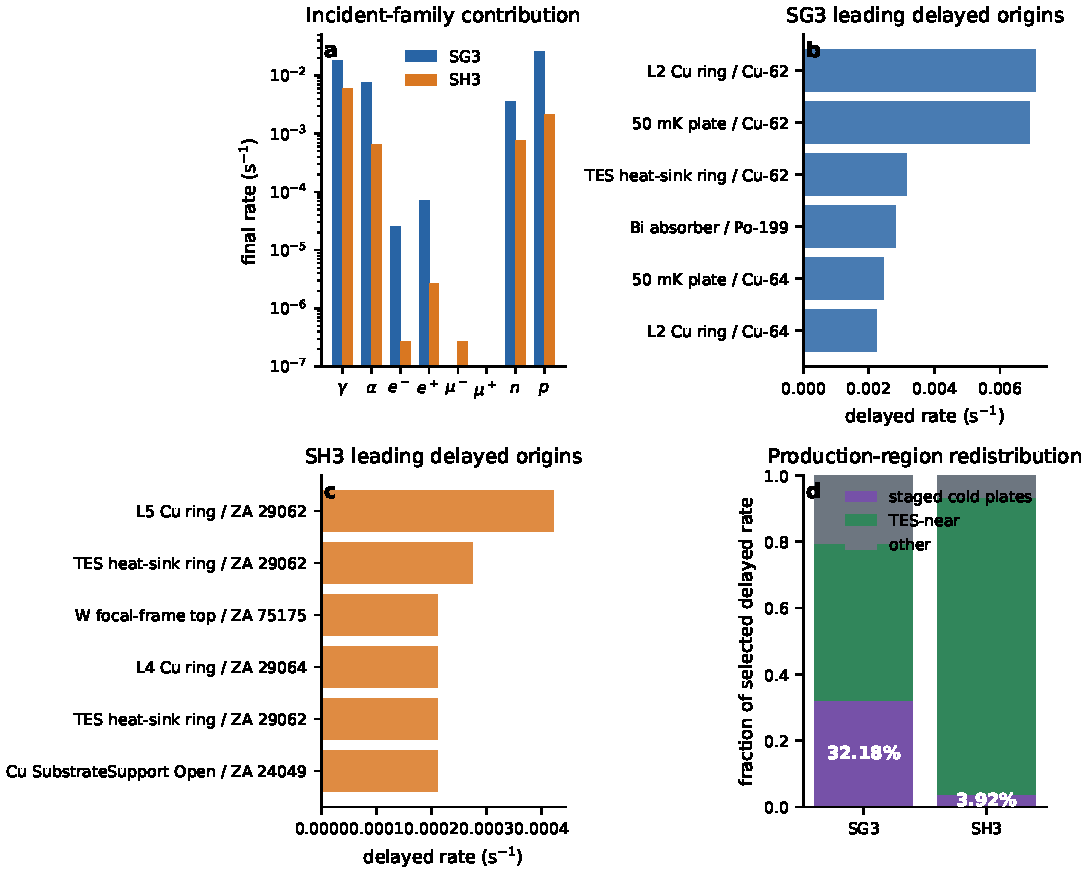
\includegraphics[width=0.98\linewidth]{figures/fig08_background_origins.pdf}
\caption{匹配 SG3 与 SH3 目录的选后本底来源。（a）按入射族分解的最终直接率。（b,c）SG3 与 SH3 的主导延迟“源体积--母核素”组。（d）选后延迟率按多级冷盘、TES 近场结构及其他结构分组。焦面移入烟囱后，多级冷端占比由 $32.18\%$ 降至 $3.92\%$。}
\label{fig:background_origin_story_zh}
\end{figure}

粒子族分解改变了参考本底的物理解释。瞬发泄漏只有宽带 $\gamma$ 样本支持，而质子诱发延迟活化是最大直接分量。SG3 的主导延迟组为 L2 铜支撑环和 50 mK 混合室板中的 $^{62}$Cu，其后是 TES 热沉环与 Bi 吸收体。因此总清单并不足够；关键量是既产生于几何强耦合位置、又能通过科学窗选择的活度。

产生区域进一步指出几何杠杆。SG3 选后延迟率中 $32.18\%$ 来自 DR 混合室与多级冷盘，另有 $47.29\%$ 来自 TES 近场结构。SH3 平移使焦面脱离冷端直接投影；多级冷端占比降至 $3.92\%$，选后延迟率由 $3.82661\times10^{-2}$ 降至 $3.62467\times10^{-3}\cps$。

\FloatBarrier

\subsection{最终侧烟囱主动屏蔽几何}
\label{subsec:optimized_shield_results_zh}

最终 SH3 将六层 TES 沿局部 $z'=-2.80$ cm 的横向烟囱轴布置。3 mm Al 壁连续连接烟囱与 DR，烟囱底部比 DR 底部高 0.25 cm；紧凑 W 框支撑焦面，三个主动 BGO 体积覆盖烟囱侧面、前端光学环和后端冷孔环。图~\ref{fig:optimized_shield_background_zh} 把该布局连接到 cut-flow 和最终组成，表~\ref{tab:final_geometry_zh} 给出输运使用的尺寸。

\begin{figure}[!ht]
\centering
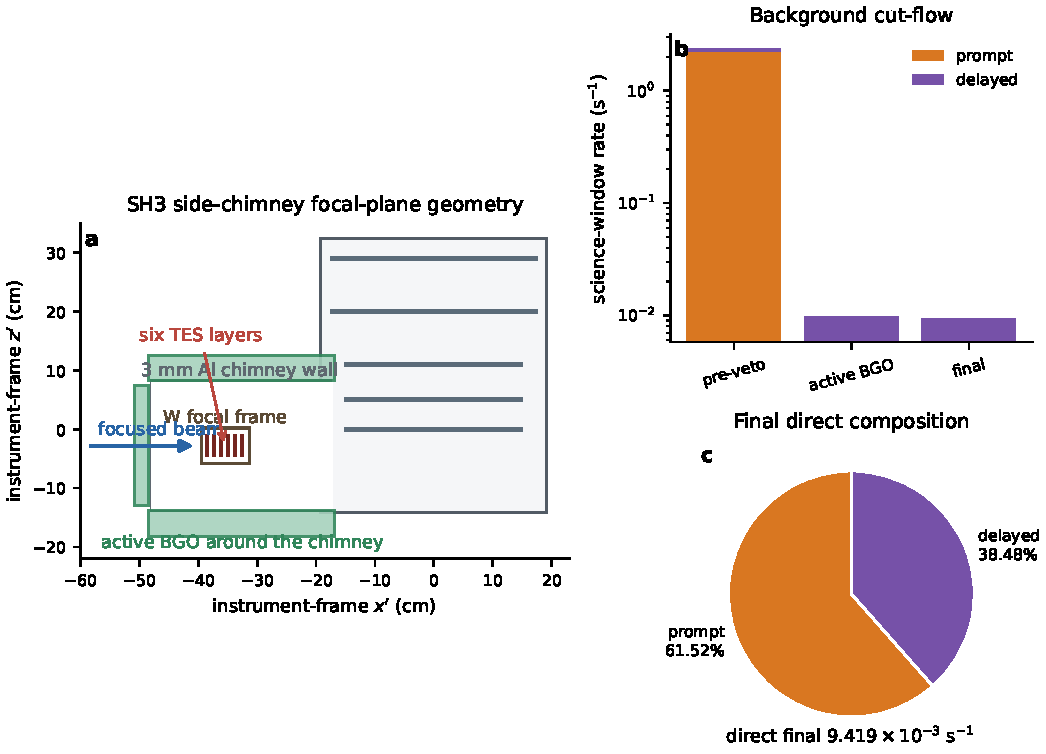
\includegraphics[width=0.92\linewidth]{figures/fig09_sh3_geometry_background.pdf}
\caption{SH3 烟囱几何与选后本底。（a）仪器坐标截面，显示横向 Al 烟囱、六层 TES、W 焦面框、聚焦光路、多级冷盘和主动 BGO。（b）瞬发与延迟直接率经过科学窗、主动 BGO 和最终拓扑阶段的变化。（c）最终直接本底 $9.41868\times10^{-3}\cps$ 的组成。}
\label{fig:optimized_shield_background_zh}
\end{figure}

\begin{table}[!ht]
\centering
\caption{最终 SH3 侧烟囱在局部仪器坐标中的几何参数。}
\label{tab:final_geometry_zh}
\footnotesize
\begin{tabular}{p{0.23\linewidth}p{0.34\linewidth}p{0.34\linewidth}}
\toprule
部件 & 最终设置 & 物理作用 \\
\midrule
Al 烟囱 & 内/外半径 10.75/11.05 cm；壁厚 3 mm & 将 TES 横向移离多级冷端区域 \\
共同轴与间隙 & $z'=-2.80$ cm；烟囱/DR 底部 $-13.85/-14.10$ cm & 连续接口并保留 0.25 cm 间隙 \\
TES 焦面 & 沿烟囱轴布置六层 Ta 像素 & 保持探测器响应和多层阻止深度 \\
W 焦面框 & 外/内方孔 6.00/5.40 cm；深 2.00 cm & 紧凑局部支撑及孔径定义 \\
冷端/光学孔 & 1.50 cm 冷孔；6.00 cm 上端光学开孔 & 保留低温服务和聚焦光束通道 \\
主动 BGO & 侧屏、前端光学环、后端冷孔环 & 环绕烟囱的逐事例反符合 \\
BGO 阈值 & 50 keV 离线沉积能；80 keV 原生触发参考 & 共同主动 veto 判据 \\
\bottomrule
\end{tabular}
\end{table}

选后面积验证表明该位移没有牺牲光学响应。最终选择后 SG3 为 $15.12324\pm0.04492\,\mathrm{cm^2}$，SH3 为 $15.08544\pm0.04503\,\mathrm{cm^2}$，故烟囱保留参考有效面积的 $99.75\%$。

\FloatBarrier

\subsection{全链本底与统计支撑}
\label{subsec:optimized_fullchain_zh}

表~\ref{tab:optimized_cutflow_zh} 以同一响应与事例序列给出 SH3 cut-flow。本底列是直接无符合值；任务计算在每个轨迹节点施加测得的公共时间因子。

\begin{table}[!ht]
\centering
\caption{SH3 经响应卷积的科学窗 cut-flow。本底为直接无符合记录数/率；信号为记录数/有效面积。}
\label{tab:optimized_cutflow_zh}
\footnotesize
\begin{tabular}{lccc}
\toprule
计算流 & 预 veto & 主动 BGO 后 & 最终拓扑/视场后 \\
\midrule
瞬发本底 & 3212 / $2.23515\cps$ & 12 / $5.79401\times10^{-3}\cps$ & 12 / $5.79401\times10^{-3}\cps$ \\
延迟活化 & 3249 / $0.127481\cps$ & 122 / $4.01926\times10^{-3}\cps$ & 111 / $3.62467\times10^{-3}\cps$ \\
总本底 & 6461 / $2.36263\cps$ & 134 / $9.81327\times10^{-3}\cps$ & 123 / $9.41868\times10^{-3}\cps$ \\
聚焦信号 & 28434 / $15.35436\,\mathrm{cm^2}$ & 28434 / $15.35436\,\mathrm{cm^2}$ & 27936 / $15.08544\,\mathrm{cm^2}$ \\
\bottomrule
\end{tabular}
\end{table}

主动 BGO 将总直接率压低至预 veto 值的 $0.4154\%$；拓扑检验再保留 BGO 选后带权率的 $95.98\%$。瞬发 $\gamma$ 为 $5.79401\times10^{-3}\cps$（61.52\%），延迟活化为 $3.62467\times10^{-3}\cps$（38.48\%）。主任务投影采用第 15 天公共时间本底 $9.280\times10^{-3}\cps$。

\begin{table}[!ht]
\centering
\caption{SH3 最终直接本底的有限输运支撑。区间为双侧 95\% Garwood 计数区间乘以分量权重；小计上端只作诊断，不是联合置信区间。}
\label{tab:optimized_component_precision_zh}
\scriptsize
\resizebox{\linewidth}{!}{%
\begin{tabular}{lrrrrr}
\toprule
分量 & 记录数 & 权重 / $\cps$ & 中心率 / $\cps$ & 95\% 区间 / $\cps$ & 总本底 / \% \\
\midrule
瞬发 $\alpha$ & 0 & $5.4193\times10^{-3}$ & 0 & $[0,1.9991\times10^{-2}]$ & 0 \\
瞬发 $e^-$ & 0 & $1.8840\times10^{-3}$ & 0 & $[0,6.9500\times10^{-3}]$ & 0 \\
瞬发 $e^+$ & 0 & $5.4388\times10^{-3}$ & 0 & $[0,2.0063\times10^{-2}]$ & 0 \\
瞬发 $\gamma$ & 12 & $4.8283\times10^{-4}$ & $5.7940\times10^{-3}$ & $[2.9939\times10^{-3},1.0121\times10^{-2}]$ & 61.516 \\
瞬发 $\mu^-$ & 0 & $1.3461\times10^{-3}$ & 0 & $[0,4.9655\times10^{-3}]$ & 0 \\
瞬发 $\mu^+$ & 0 & $3.9779\times10^{-3}$ & 0 & $[0,1.4674\times10^{-2}]$ & 0 \\
瞬发 $n$ & 0 & $5.5440\times10^{-3}$ & 0 & $[0,2.0451\times10^{-2}]$ & 0 \\
瞬发 $p$ & 0 & $1.2360\times10^{-2}$ & 0 & $[0,4.5595\times10^{-2}]$ & 0 \\
瞬发小计 & 12 & -- & $5.7940\times10^{-3}$ & 上端和 $1.4281\times10^{-1}$ & 61.516 \\
延迟 $\alpha$ & 19 & $3.4284\times10^{-5}$ & $6.5139\times10^{-4}$ & $[3.9218\times10^{-4},1.0172\times10^{-3}]$ & 6.916 \\
延迟 $e^-$ & 1 & $2.6633\times10^{-7}$ & $2.6633\times10^{-7}$ & $[6.7429\times10^{-9},1.4839\times10^{-6}]$ & 0.003 \\
延迟 $e^+$ & 4 & $6.7536\times10^{-7}$ & $2.7015\times10^{-6}$ & $[7.3606\times10^{-7},6.9168\times10^{-6}]$ & 0.029 \\
延迟 $\gamma$ & 52 & $2.0320\times10^{-6}$ & $1.0567\times10^{-4}$ & $[7.8917\times10^{-5},1.3857\times10^{-4}]$ & 1.122 \\
延迟 $\mu^-$ & 4 & $6.8409\times10^{-8}$ & $2.7364\times10^{-7}$ & $[7.4557\times10^{-8},7.0062\times10^{-7}]$ & 0.003 \\
延迟 $\mu^+$ & 0 & $3.9662\times10^{-9}$ & 0 & $[0,1.4631\times10^{-8}]$ & 0 \\
延迟 $n$ & 11 & $6.8532\times10^{-5}$ & $7.5385\times10^{-4}$ & $[3.7632\times10^{-4},1.3488\times10^{-3}]$ & 8.004 \\
延迟 $p$ & 20 & $1.0553\times10^{-4}$ & $2.1105\times10^{-3}$ & $[1.2892\times10^{-3},3.2595\times10^{-3}]$ & 22.408 \\
延迟小计 & 111 & -- & $3.6247\times10^{-3}$ & 上端和 $5.7733\times10^{-3}$ & 38.484 \\
\midrule
总本底 & 123 & -- & $9.4187\times10^{-3}$ & 分量上端和 $1.4858\times10^{-1}$ & 100.000 \\
\bottomrule
\end{tabular}}
\end{table}

分量表揭示有限输运支撑仍稀疏的位置，但主流量阈值不确定度不是其端点之和。匹配的 delta 方法预算给出 18.67\% 本底输运项、1.13\% 时间轴项、0.30\% 选后面积项以及可忽略的偶然符合探针项；传播后 SH3 高斯 $3\sigma$ 流量阈值的相对 $1\sigma$ 不确定度为 9.36\%。

\FloatBarrier

\subsection{最终几何的任务性能}
\label{subsec:final_mission_performance_zh}

图~\ref{fig:optimized_mission_significance_zh} 比较匹配的 81 节点折叠。20 d 时，SG3 累计 1635.07 个信号和 86806.00 个本底计数，SH3 累计 1678.14 和 15551.68 个；高斯显著度分别为 5.55 和 13.46，Asimov 值为 5.53 和 13.22。

\begin{figure}[!ht]
\centering
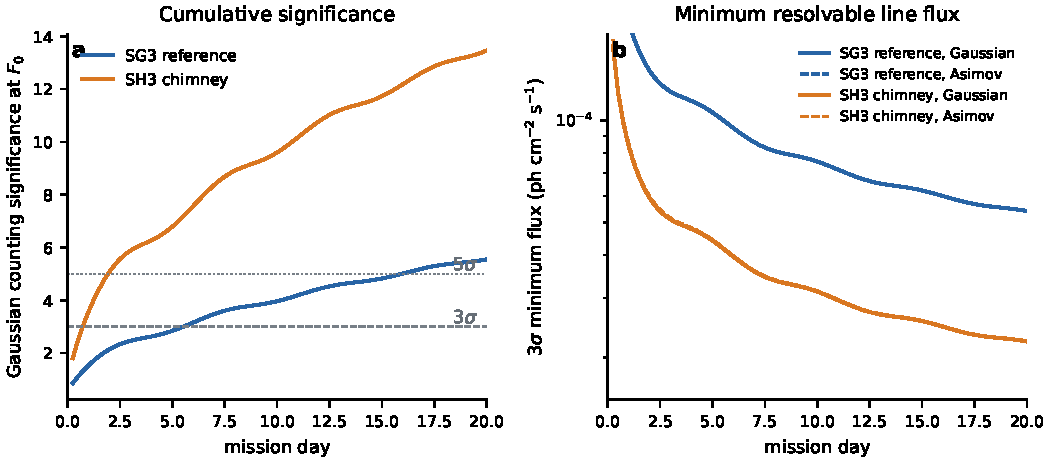
\includegraphics[width=0.98\linewidth]{figures/fig10_mission_performance.pdf}
\caption{SG3 参考与 SH3 烟囱几何的匹配 81 节点任务性能。（a）$F_0=10^{-4}\phcms$ 下的高斯计数显著度，水平线标出 $3\sigma$ 与 $5\sigma$。（b）高斯和 Asimov $3\sigma$ 最小可分辨流量。两条曲线采用相同源、响应、选择、计时及大气透过约定。}
\label{fig:optimized_mission_significance_zh}
\end{figure}

\begin{table}[!ht]
\centering
\caption{SG3 参考与 SH3 烟囱几何的匹配任务投影；括号内为高斯 $3\sigma$ 流量阈值的传播 $1\sigma$ 统计不确定度。}
\label{tab:primary_sensitivity_zh}
\footnotesize
\resizebox{\linewidth}{!}{%
\begin{tabular}{lrr}
\toprule
量 & SG3 参考 & SH3 烟囱 \\
\midrule
选后有效面积 / $\mathrm{cm^2}$ & $15.12324\pm0.04492$ & $15.08544\pm0.04503$ \\
第 15 天本底 / $\cps$ & $5.12802\times10^{-2}$ & $9.2800\times10^{-3}$ \\
第 15 天 $F_0$ 信号 / $\cps$ & $9.53616\times10^{-4}$ & $9.79040\times10^{-4}$ \\
20 d 本底计数 & 86806.00 & 15551.68 \\
20 d $F_0$ 信号计数 & 1635.07 & 1678.14 \\
$Z_{20\mathrm d}$，高斯 / Asimov & 5.550 / 5.532 & 13.457 / 13.225 \\
$T_{3\sigma}$，高斯 / Asimov / d & 5.525 / 5.555 & 0.724 / 0.753 \\
$T_{5\sigma}$，高斯 / Asimov / d & 15.932 / 16.010 & 1.935 / 2.030 \\
$F_{3\sigma}(20\,\mathrm d)$，高斯 / Asimov / $\phcms$ &
$(5.406\pm0.401)\times10^{-5}$ / $5.415\times10^{-5}$ &
$(2.229\pm0.209)\times10^{-5}$ / $2.238\times10^{-5}$ \\
\bottomrule
\end{tabular}}
\end{table}

SH3 本底为 SG3 的 $18.10\%$，选后有效面积为参考值的 $99.75\%$。高斯 20 d 最小流量是 SG3 阈值的 $41.24\%$，相当于改善 2.43 倍；端点处高斯与 Asimov 结果接近，说明该比较不是大本底近似造成的假象。

\section{讨论}
\label{sec:discussion}

主要结果是几何变化的完整物理解释。SG3 的 TES 位于多级冷盘下方，该区域的选后延迟活度提供 32.18\% 的科学窗延迟率。SH3 将同一六层焦面横向移入 BGO 包围的烟囱，使该比例降至 3.92\%；有效面积变化不超过 0.25\%，成熟本底则降低 5.53 倍。几何、选后事例来源和任务灵敏度因而是同一结果的三个层面。

这一分析顺序与近期仪器本底研究一致。COSI 在详细气球载荷中分别输运瞬发与活化分量，并与飞行数据比较其能谱和时间行为 \cite{Gallego2025Balloon}；DIXE 同样从详细 TES 载荷出发，追问哪些入射粒子、产生区域和物理过程构成探测谱 \cite{Tian2026DIXE}。本工作中总清单与选后来源的区别尤其关键：主导选后组集中在局部 Cu 与近场结构，因此只依据总活度会遗漏真正的几何杠杆。

最终分量组成还分离了仪器各层的作用。主动 BGO 提供主要抑制，将 SH3 科学窗直接率由 2.36263 降至 $9.8133\times10^{-3}\cps$；宽松拓扑检验移除较小残余，同时保留 98.25\% 的科学窗信号。剩余瞬发项来自宽带大气 $\gamma$，延迟项来自全部八类入射族产生的活化。

该望远镜的观测角色与测量核球、银盘及更广银河发射的 INTEGRAL/SPI 和 COSI 互补 \cite{Siegert2016AA,Kierans2020,Siegert2020COSI,Yoneda2025,Karwin2023}。Laue 透镜--TES 概念以天空覆盖换取集中束流和亚 keV 科学窗，适合紧致 511 keV 源、未分辨中心分量及定点后随观测。表~\ref{tab:primary_sensitivity_zh} 量化的是持续在源、窄线的 20 d 参考情形。

\subsection{适用范围与下一步}
\label{subsec:limitations}

任务数值是探测器--低温系统几何及合成连续在源轨迹的统计投影。计算采用 50 keV 离线 BGO 沉积能阈值、探测器级拓扑检验、全部八族瞬发和全部八族活化。BGO 判据是理想离线沉积能阈值，并非实测硬件触发效率；80 keV 仅为原生触发参考。Laue 光学与气球平台本底不在当前探测器--低温系统预算内。辐射场、截面、标定、重建和指向系统学也不在传播统计不确定度内。

当前精度主要受选后输运事件数有限且权重不等限制。后续应增加瞬发 $\gamma$ 和主导延迟族支撑，重复产生位置抽样以检验空间收敛，以实际飞行计划和可见性历史替换合成轨迹，并标定能量响应与 BGO 触发效率。随后可使用聚焦斑和控制区构建空间--能谱似然，同时剖面化本底扰动参数 \cite{Cowan2011}；这会扩展当前“来源--几何”逻辑，但不改变已经闭合的 SG3--SH3 同口径比较。

\subsection{结论}
\label{sec:conclusions}

SG3 参考指出，多级冷端及其附近活化结构是选后延迟本底的重要来源。将六层 TES 焦面移入 SH3 横向烟囱后，冷端占比由 32.18\% 降至 3.92\%，同时保留 $99.75\%$ 的选后有效面积。第 15 天 SH3 得到 $B=9.280\times10^{-3}\cps$，在 $F_0=10^{-4}\phcms$ 下 $S=9.790\times10^{-4}\cps$；沿固定 $45^\circ$ 的 20 d 轨迹，高斯与 Asimov 显著度为 13.46 和 13.22，高斯 $3\sigma$ 阈值为 $(2.229\pm0.209)\times10^{-5}\phcms$。相对 SG3，匹配阈值改善约 2.43 倍，表明粒子族、母核素和产生位置分辨的本底信息可以直接转化为焦面几何和任务尺度 511 keV 性能预测。

\section*{数据与软件可用性}
正式发表前，应通过带版本号的公共代码仓库或机构存档提供复现本文图表所需的几何和源定义、随机性约定、分析与制图脚本、LaTeX 源文件及派生验证产物。

\section*{声明}
\textbf{经费来源} 投稿前补充。

\textbf{利益冲突} 投稿前补充。

\textbf{作者贡献} 投稿前补充。

\textbf{伦理审批与参与同意} 不适用。

\begin{thebibliography}{99}

\bibitem{Prantzos2011}
N. Prantzos, C. Boehm, A.M. Bykov, R. Diehl, K. Ferriere, N. Guessoum, P. Jean, J. Knoedlseder, A. Marcowith, I.V. Moskalenko, A. Strong, G. Weidenspointner, The 511 keV emission from positron annihilation in the Galaxy, Rev. Mod. Phys. 83 (2011) 1001--1056, doi:10.1103/RevModPhys.83.1001.

\bibitem{Jean2006}
P. Jean, J. Knoedlseder, V. Lonjou, M. Allain, J.-P. Roques, G.K. Skinner, B.J. Teegarden, G. Vedrenne, P. von Ballmoos, B. Cordier, P. Caraveo, R. Diehl, P. Durouchoux, P. Leleux, R. Schanne, G. Weidenspointner, Spectral analysis of the Galactic $e^+e^-$ annihilation emission, Astron. Astrophys. 445 (2006) 579--589, doi:10.1051/0004-6361:20053765.

\bibitem{Kierans2020}
C.A. Kierans, S.E. Boggs, A. Zoglauer, A.W. Lowell, C. Sleator, J. Beechert, T.J. Brandt, P. Jean, H. Lazar, J. Roberts, T. Siegert, J.A. Tomsick, P. von Ballmoos, Detection of the 511 keV Galactic positron annihilation line with COSI, Astrophys. J. 895 (2020) 44, doi:10.3847/1538-4357/ab89a9.

\bibitem{Siegert2016AA}
T. Siegert, R. Diehl, G. Khachatryan, M.G.H. Krause, F. Guglielmetti, J. Greiner, A.W. Strong, X. Zhang, Gamma-ray spectroscopy of positron annihilation in the Milky Way, Astron. Astrophys. 586 (2016) A84, doi:10.1051/0004-6361/201527510.

\bibitem{Siegert2016V404}
T. Siegert, R. Diehl, J. Greiner, M.G.H. Krause, A.M. Beloborodov, M. Cadolle Bel, F. Guglielmetti, J. Rodriguez, A.W. Strong, X. Zhang, Positron annihilation signatures associated with the outburst of the microquasar V404 Cygni, Nature 531 (2016) 341--343, doi:10.1038/nature16978.

\bibitem{Knodlseder2005AllSky}
J. Knoedlseder, P. Jean, V. Lonjou, G. Weidenspointner, N. Guessoum, R. Diehl, W. Gillard, M.J. Harris, G.K. Skinner, P. von Ballmoos, G. Vedrenne, P. Caraveo, B. Cordier, V. Schoenfelder, B.J. Teegarden, The all-sky distribution of 511 keV electron-positron annihilation emission, Astron. Astrophys. 441 (2005) 513--532, doi:10.1051/0004-6361:20042063.

\bibitem{Yoneda2025}
H. Yoneda, T. Siegert, S. Mittal, Imaging the positron annihilation line with 20 years of INTEGRAL/SPI observations, arXiv:2509.01066, 2025.

\bibitem{Siegert2020COSI}
T. Siegert, S.E. Boggs, J.A. Tomsick, A.C. Zoglauer, C.A. Kierans, C.C. Sleator, J. Beechert, T.J. Brandt, P. Jean, H. Lazar, A.W. Lowell, J.M. Roberts, P. von Ballmoos, Imaging the 511 keV positron annihilation sky with COSI, Astrophys. J. 897 (2020) 45, doi:10.3847/1538-4357/ab9607.

\bibitem{Siegert2019Kinematics}
T. Siegert, R. Diehl, G. Khachatryan, M.G.H. Krause, F. Guglielmetti, J. Greiner, A.W. Strong, X. Zhang, Constraints on positron annihilation kinematics in the inner Galaxy, Astron. Astrophys. 627 (2019) A126, doi:10.1051/0004-6361/201833856.

\bibitem{DeCesare2011}
G. De Cesare, Searching for the 511 keV annihilation line from galactic compact objects with the IBIS gamma ray telescope, Astron. Astrophys. 531 (2011) A56, doi:10.1051/0004-6361/201116516.

\bibitem{Barriere2009Laue}
N.M. Barriere, L. Natalucci, N. Abrosimov, P. von Ballmoos, P. Bastie, P. Courtois, M. Jentschel, J. Knodlseder, J. Rousselle, P. Ubertini, Soft gamma-ray optics: new Laue lens design and performance estimates, arXiv:0910.0488, 2009.

\bibitem{Barriere2011LauePrototype}
N.M. Barriere, J.A. Tomsick, S.E. Boggs, A. Lowell, P. von Ballmoos, Developing a second generation Laue lens prototype: high reflectivity crystals and accurate assembly, arXiv:1111.6700, 2011.

\bibitem{Weidenspointner2006MAX}
G. Weidenspointner, C.B. Wunderer, N. Barriere, A. Zoglauer, P. von Ballmoos, Monte Carlo study of detector concepts for the MAX Laue Lens gamma-ray telescope, arXiv:astro-ph/0603152, 2006.

\bibitem{Shirazi2023}
F. Shirazi, E. Gau, M.A. Hossen, D. Becker, D. Schmidt, D. Swetz, D. Bennett, D. Braun, F. Kislat, J. Gard, J. Mates, J. Weber, N.R. Cavero, S. Chun, L. Lisalda, A. West, B. Dev, F. Ferrer, R. Bose, J. Ullom, H. Krawczynski, The 511-CAM Mission: A pointed 511 keV gamma-ray telescope with a focal plane detector made of stacked transition edge sensor microcalorimeter arrays, J. Astron. Telesc. Instrum. Syst. 9 (2023) 024006, doi:10.1117/1.JATIS.9.2.024006.

\bibitem{Zhang2022TESGamma}
S. Zhang, J.-K. Xia, T. Sun, et al., Transition edge sensor based detector: from X-ray to gamma-ray, arXiv:2204.00010, 2022.

\bibitem{Hu2026}
K. Hu, M. Fritts, D. Becker, D. Schmidt, F. Zhou, A. Dasgupta, F. Kislat, M. Keller, S. Chun, A.G. Detoito, E. Gau, X. Jin, D. Bennett, D. Braun, J. Gard, J.A.B. Mates, J. Nobles, D. Radomski, N. Rodriguez Cavero, R. Snodgrass, D. Swetz, J. Ullom, S. Vengalil Menon, J. Weber, K. Wimalasena, H. Krawczynski, Design of a mission to measure the shape and substructure of the 511 keV gamma-ray line from the center of the Milky Way, J. Astron. Telesc. Instrum. Syst. 12 (2026) 025002, doi:10.1117/1.JATIS.12.2.025002.

\bibitem{Gallego2025Balloon}
S. Gallego, U. Oberlack, J. Lommler, C.M. Karwin, A. Zoglauer, P. Jean, P. von Ballmoos, C. Kierans, C.C. Sleator, J.A. Tomsick, S.E. Boggs, Bottom-up background simulations of the 2016 COSI balloon flight, Astrophys. J. 986 (2025) 116, doi:10.3847/1538-4357/add6a0.

\bibitem{Tian2026DIXE}
R. Tian, J. Mao, J. Liu, H. Jin, W. Cui, Simulation of non-X-ray background for the DIffuse X-ray Explorer (DIXE) mission, arXiv:2604.13569, 2026.

\bibitem{Caputo2017}
R. Caputo, F. Kislat, J. Racusin, on behalf of the AMEGO Team, AMEGO: Simulations of the instrument performance, Proc. 35th International Cosmic Ray Conference, PoS(ICRC2017) 783 (2018), doi:10.22323/1.301.0783.

\bibitem{Gottardi2021TESReview}
L. Gottardi, K. Nagayoshi, A review of X-ray microcalorimeters based on superconducting transition edge sensors for astrophysics and particle physics, Applied Sciences 11 (2021) 3793, doi:10.3390/app11093793.

\bibitem{Xie2026AlMn}
L. Xie, Y. Zhang, Z. Li, Z. Liu, S. Shu, J. Zhou, X. Li, H. Li, H. Gao, Y. Gu, X. Lu, Y. Zhao, C. Liu, Beyond one-thousandth energy resolution with an AlMn TES detector, arXiv:2602.11728, 2026.

\bibitem{Vavagiakis2017AlMnMagnetic}
E.M. Vavagiakis, S.W. Henderson, K. Zheng, H.-M. Cho, N.F. Cothard, B. Dober, S.M. Duff, P.A. Gallardo, G. Hilton, J. Hubmayr, K.D. Irwin, B.J. Koopman, D. Li, F. Nati, M.D. Niemack, C.D. Reintsema, S. Simon, J.R. Stevens, A. Suzuki, B. Westbrook, Magnetic sensitivity of AlMn TESes and shielding considerations for next-generation CMB surveys, arXiv:1710.08456, 2017.

\bibitem{NISTXCOM}
J.H. Hubbell, S.M. Seltzer, XCOM: Photon Cross Section Database, NIST Standard Reference Database 8 (XGAM), National Institute of Standards and Technology, doi:10.18434/T48G6X.

\bibitem{Sturner2003}
S.J. Sturner, C.R. Shrader, G. Weidenspointner, B.J. Teegarden, D. Attie, B. Cordier, R. Diehl, C. Ferguson, P. Jean, A. von Kienlin, P. Paul, F. Sanchez, S. Schanne, P. Sizun, G. Skinner, C.B. Wunderer, Monte Carlo simulations and generation of the SPI response, Astron. Astrophys. 411 (2003) L81--L84, doi:10.1051/0004-6361:20031171.

\bibitem{Agostinelli2003}
S. Agostinelli, J. Allison, K. Amako, et al., Geant4---a simulation toolkit, Nucl. Instrum. Methods Phys. Res. A 506 (2003) 250--303, doi:10.1016/S0168-9002(03)01368-8.

\bibitem{Allison2016}
J. Allison, K. Amako, J. Apostolakis, et al., Recent developments in Geant4, Nucl. Instrum. Methods Phys. Res. A 835 (2016) 186--225, doi:10.1016/j.nima.2016.06.125.

\bibitem{SanchezDelRio2011XOP}
M. Sanchez del Rio, R.J. Dejus, XOP v2.4: recent developments of the x-ray optics software toolkit, Proc. SPIE 8141 (2011) 814115, doi:10.1117/12.893911.

\bibitem{Guan2023BraggReflection}
F. Guan, M. Asai, D.A. Bartkoski, M. Kleckner, Z. Harel, M. Salehpour, Adding the X-ray Bragg reflection physical process in crystal to the Geant4 Monte Carlo simulation toolkit, part I: reflection from a crystal slab, Precision Radiation Oncology 7(1) (2023) 59--66.

\bibitem{Reiazi2025G4BraggReflection}
R. Reiazi, D. Lee, D. Bartkoski, M. Kleckner, M. Salehpour, G4BraggReflection for accurate modeling of Bragg reflection in perfect and mosaic crystals, J. Phys. D: Appl. Phys. 58 (2025) 295102, doi:10.1088/1361-6463/aded1d.

\bibitem{Zoglauer2006}
A. Zoglauer, R. Andritschke, F. Schopper, MEGAlib: The Medium Energy Gamma-ray Astronomy Library, New Astron. Rev. 50 (2006) 629--632, doi:10.1016/j.newar.2006.06.049.

\bibitem{Sato2015EXPACS}
T. Sato, Analytical model for estimating terrestrial cosmic ray fluxes nearly anytime and anywhere in the world: extension of PARMA/EXPACS, PLoS ONE 10 (2015) e0144679, doi:10.1371/journal.pone.0144679.

\bibitem{Sato2016PARMA4}
T. Sato, Analytical model for estimating the zenith angle dependence of terrestrial cosmic ray fluxes, PLoS ONE 11 (2016) e0160390, doi:10.1371/journal.pone.0160390.

\bibitem{Mahoney1981Atmospheric}
W.A. Mahoney, J.C. Ling, A.S. Jacobson, HEAO 3 measurements of the atmospheric positron annihilation line, J. Geophys. Res. 86 (1981) 11098--11104, doi:10.1029/JA086iA13p11098.

\bibitem{Harris2003Atmospheric}
M.J. Harris, G.H. Share, M.D. Leising, Spatial and temporal variability of the gamma radiation from Earth's atmosphere during a solar cycle, J. Geophys. Res. Space Phys. 108 (2003) 1435, doi:10.1029/2003JA009958.

\bibitem{Kondev2021NUBASE}
F.G. Kondev, M. Wang, W.J. Huang, S. Naimi, G. Audi, The NUBASE2020 evaluation of nuclear physics properties, Chinese Phys. C 45 (2021) 030001, doi:10.1088/1674-1137/abddae.

\bibitem{Kierans2017}
C.A. Kierans, S.E. Boggs, J.-L. Chiu, A. Lowell, C. Sleator, J.A. Tomsick, A. Zoglauer, M. Amman, H.-K. Chang, C.-H. Tseng, C.-Y. Yang, C.-H. Lin, P. Jean, P. von Ballmoos, The 2016 Super Pressure Balloon flight of the Compton Spectrometer and Imager, arXiv:1701.05558, 2017.

\bibitem{Karwin2023}
C.M. Karwin, T. Siegert, J. Beechert, J.A. Tomsick, T.A. Porter, M. Negro, C. Kierans, M. Ajello, I. Martinez Castellanos, A. Shih, A. Zoglauer, S.E. Boggs, Probing the Galactic diffuse continuum emission with COSI, arXiv:2310.12206, 2023.

\bibitem{Cowan2011}
G. Cowan, K. Cranmer, E. Gross, O. Vitells, Asymptotic formulae for likelihood-based tests of new physics, Eur. Phys. J. C 71 (2011) 1554, doi:10.1140/epjc/s10052-011-1554-0.

\end{thebibliography}
\end{document}
